
\documentclass[letter]{article}
\usepackage[utf8]{inputenc}
\usepackage[margin=1in]{geometry}
\usepackage{tikz}
\usepackage{ulem}
\usepackage{graphics}
\usepackage{sidecap}
\usepackage{wrapfig}
\usepackage[toc,page]{appendix}
\usepackage{caption}
\usepackage{amssymb}
\usepackage{amsmath}
\usepackage{algorithmicx}
\usepackage{algpseudocode}

\usepackage{url,graphicx,tabularx,array,geometry,amsmath,tikz}
\usepackage{algorithm}% http://ctan.org/pkg/algorithms
\usepackage{algpseudocode}% http://ctan.org/pkg/algorithmicx
\usepackage{listings}
\usetikzlibrary{arrows}
\newenvironment{myindentpar}[1]% %indent whole paragraph when needed
 {\begin{list}{}%
         {\setlength{\leftmargin}{#1}}%
         \item[]%
 }
 {\end{list}}

\usepackage{hyperref}
\usepackage{parskip}

\hypersetup{
    colorlinks,%
    citecolor=black,%
    filecolor=black,%
    linkcolor=black,%
    urlcolor=black
}

\def\dashuline{\bgroup 
  \ifdim\ULdepth=\maxdimen  % Set depth based on font, if not set already
	  \settodepth\ULdepth{(j}\advance\ULdepth.4pt\fi
  \markoverwith{\kern.15em
	\vtop{\kern\ULdepth \hrule width .3em}%
	\kern.15em}\ULon}
\setlength\parindent{2em}

\newcounter{foot}
\setcounter{foot}{1}
\lstset{
  basicstyle=\small,
  stringstyle=\ttfamily,
  numbers=left,
  numberstyle=\tiny,
  stepnumber=1, 
  numbersep=5pt,
  language=R }

\author{Olga Prilepova, Christopher Patton, Alexander Rumbaugh, \\ John Chen, Thomas Provan}

\date{\today}
\title{ECS256 - Homework III}
	
\begin{document}
\maketitle

\subsection*{Problem 1.a}
First, we'll derive $\pi_i$. The definition of the tree searching markov model leads to the 
following set of balance equations for the long-run state probabilities: 
$$ \pi_i = \pi_{i-1}q_{i-1} = \pi_0 \prod_{j=0}^{i-1}{q_j} \quad \text{ for $i\ge 1$, and } $$
$$ \pi_0 = \sum_{i=1}^\infty{\pi_i(1-q_i)} \quad \text{ for $i=0$. } $$ 
This definition for $\pi_0$ is a bit unweildy. Since the chain is positive recurrent, we can 
also think of this quantity as one over the expected recurrance time, as in eq. (10.63) in 
the book: 
\begin{equation*}
  \begin{aligned}
         \pi_0 &= \frac{1}{E(T_{0,0})} \\  
    E(T_{0,0}) &= 1 + \sum_{k \ne 0}{p_{0,k}E(T_{k,0})} \quad \text{ By eq. (10.65)} \\
               &= 1 + p_{0,1}E(T_{1,0}) \\
               &= 1 + p_{0,1}(1 + \sum_{k \ne 0}{p_{1,k}E(T_{k,0})}) \\ 
               &= 1 + p_{0,1}(1 + p_{1,2}E(T_{2,0})) \\
               &= 1 + p_{0,1}(1 + p_{1,2}(1 + \sum_{k \ne 0}{p_{2,k}E(T_{k,0})})) \\
               &= 1 + p_{0,1}(1 + p_{1,2}(1 + p_{2,3}E(T_{3,0}))) 
  \end{aligned}
\end{equation*}
and so on. This unravels into a familiar closed form:   
\begin{equation*}
  \begin{aligned}
      E(T_{0,0}) &= 1 + q_0(1 + q_1(1 + q_2(1 + \dots ) \dots ))) \\ 
                 &= 1 + q_0 + q_0q_1 + q_0q_1q_2 + \dots \\
                 &= 1 + \sum_{i=1}^\infty{\big[\prod_{j=0}^{i-1}{q_j}\big]}
  \end{aligned}
\end{equation*}
If the model is positive recurrent, then there exists some value $R$ such that
$$ R = \sum_{i=1}^\infty{\big[\prod_{j=0}^{i-1}{q_j}\big]} < \infty. $$
Thus, 
$$ \pi_i = \frac{\prod_{j=0}^{i-1}{q_j}}{1 + R} \quad \text{ for $i \ge 0$. } $$


Next, $E(T_{i,0})$ follows a similar pattern. 
\begin{equation*}
  \begin{aligned}
      E(T_{i,0}) &= 1 + \sum_{k \ne 0}{p_{i,k}E(T_{k,0})} \\ 
                 &= 1 + p_{i,i+1}E(T_{j+1,0}) \\
                 &= 1 + q_i + q_iq_{i+1} + q_iq_{i+1}q_{i+2} + \dots \\
                 &= 1 + \sum_{j=i}^\infty{\Big[ \prod_{k=i}^{j}{q_k} \Big]}.
  \end{aligned}
\end{equation*}


\subsection*{Problem 1.b}
If $q_i = 0.5$ for all $i$, then $R$ is a geometric series that indeed converges. 
$$ \pi_2 = \frac{0.5 \cdot 0.5}{1 + \sum_{i=1}^\infty{0.5^{i-1}}} = 
           \frac{0.25}{1+2} \approx 0.083. $$

$$ E(T_{2,0}) = 1 + \sum_{j=2}^\infty{0.5^{j-2}} 
              = 1 + \sum_{j=1}^\infty{0.5^{j-1}} = 1 + 2 = 3. $$

\subsection*{Problem 1.c}
The rate of backtracking, in terms of the stationary probabilities $\pi_i$, is simply
$$ \sum_{i=1}^\infty{\pi_i(1 - q_i)}. $$


\subsection*{Problem 2.a}
In this problem, we are given the task of generating a method-of-stages approximation of a distribution, given its quantile function.  To accomplish the approximation, we seek to combine a set of erlang distributions and receive the approximation as the sum of the erlang distributions.

\subsection*{Problem 2.b}

Using the \textbf{ermixobj} object generated in Problem 2.a, we are able to generate a set of \textbf{nmix} erlang distributions with
parameters given as:
  Shape = \textbf{r}
  Rate = \textbf{lamb}
  
The combination of all nmix erlang distributions yields our method-of-stages approximation of the quantile function
fed into erlangmix() in Problem 2.a.

Here, we explored the effect of different values of r and nmix on the approximation.

\begin{figure}[H]
\centering
\newpage
\Large{For a uniform distribution with minimum = 10, maximum = 15:}\\
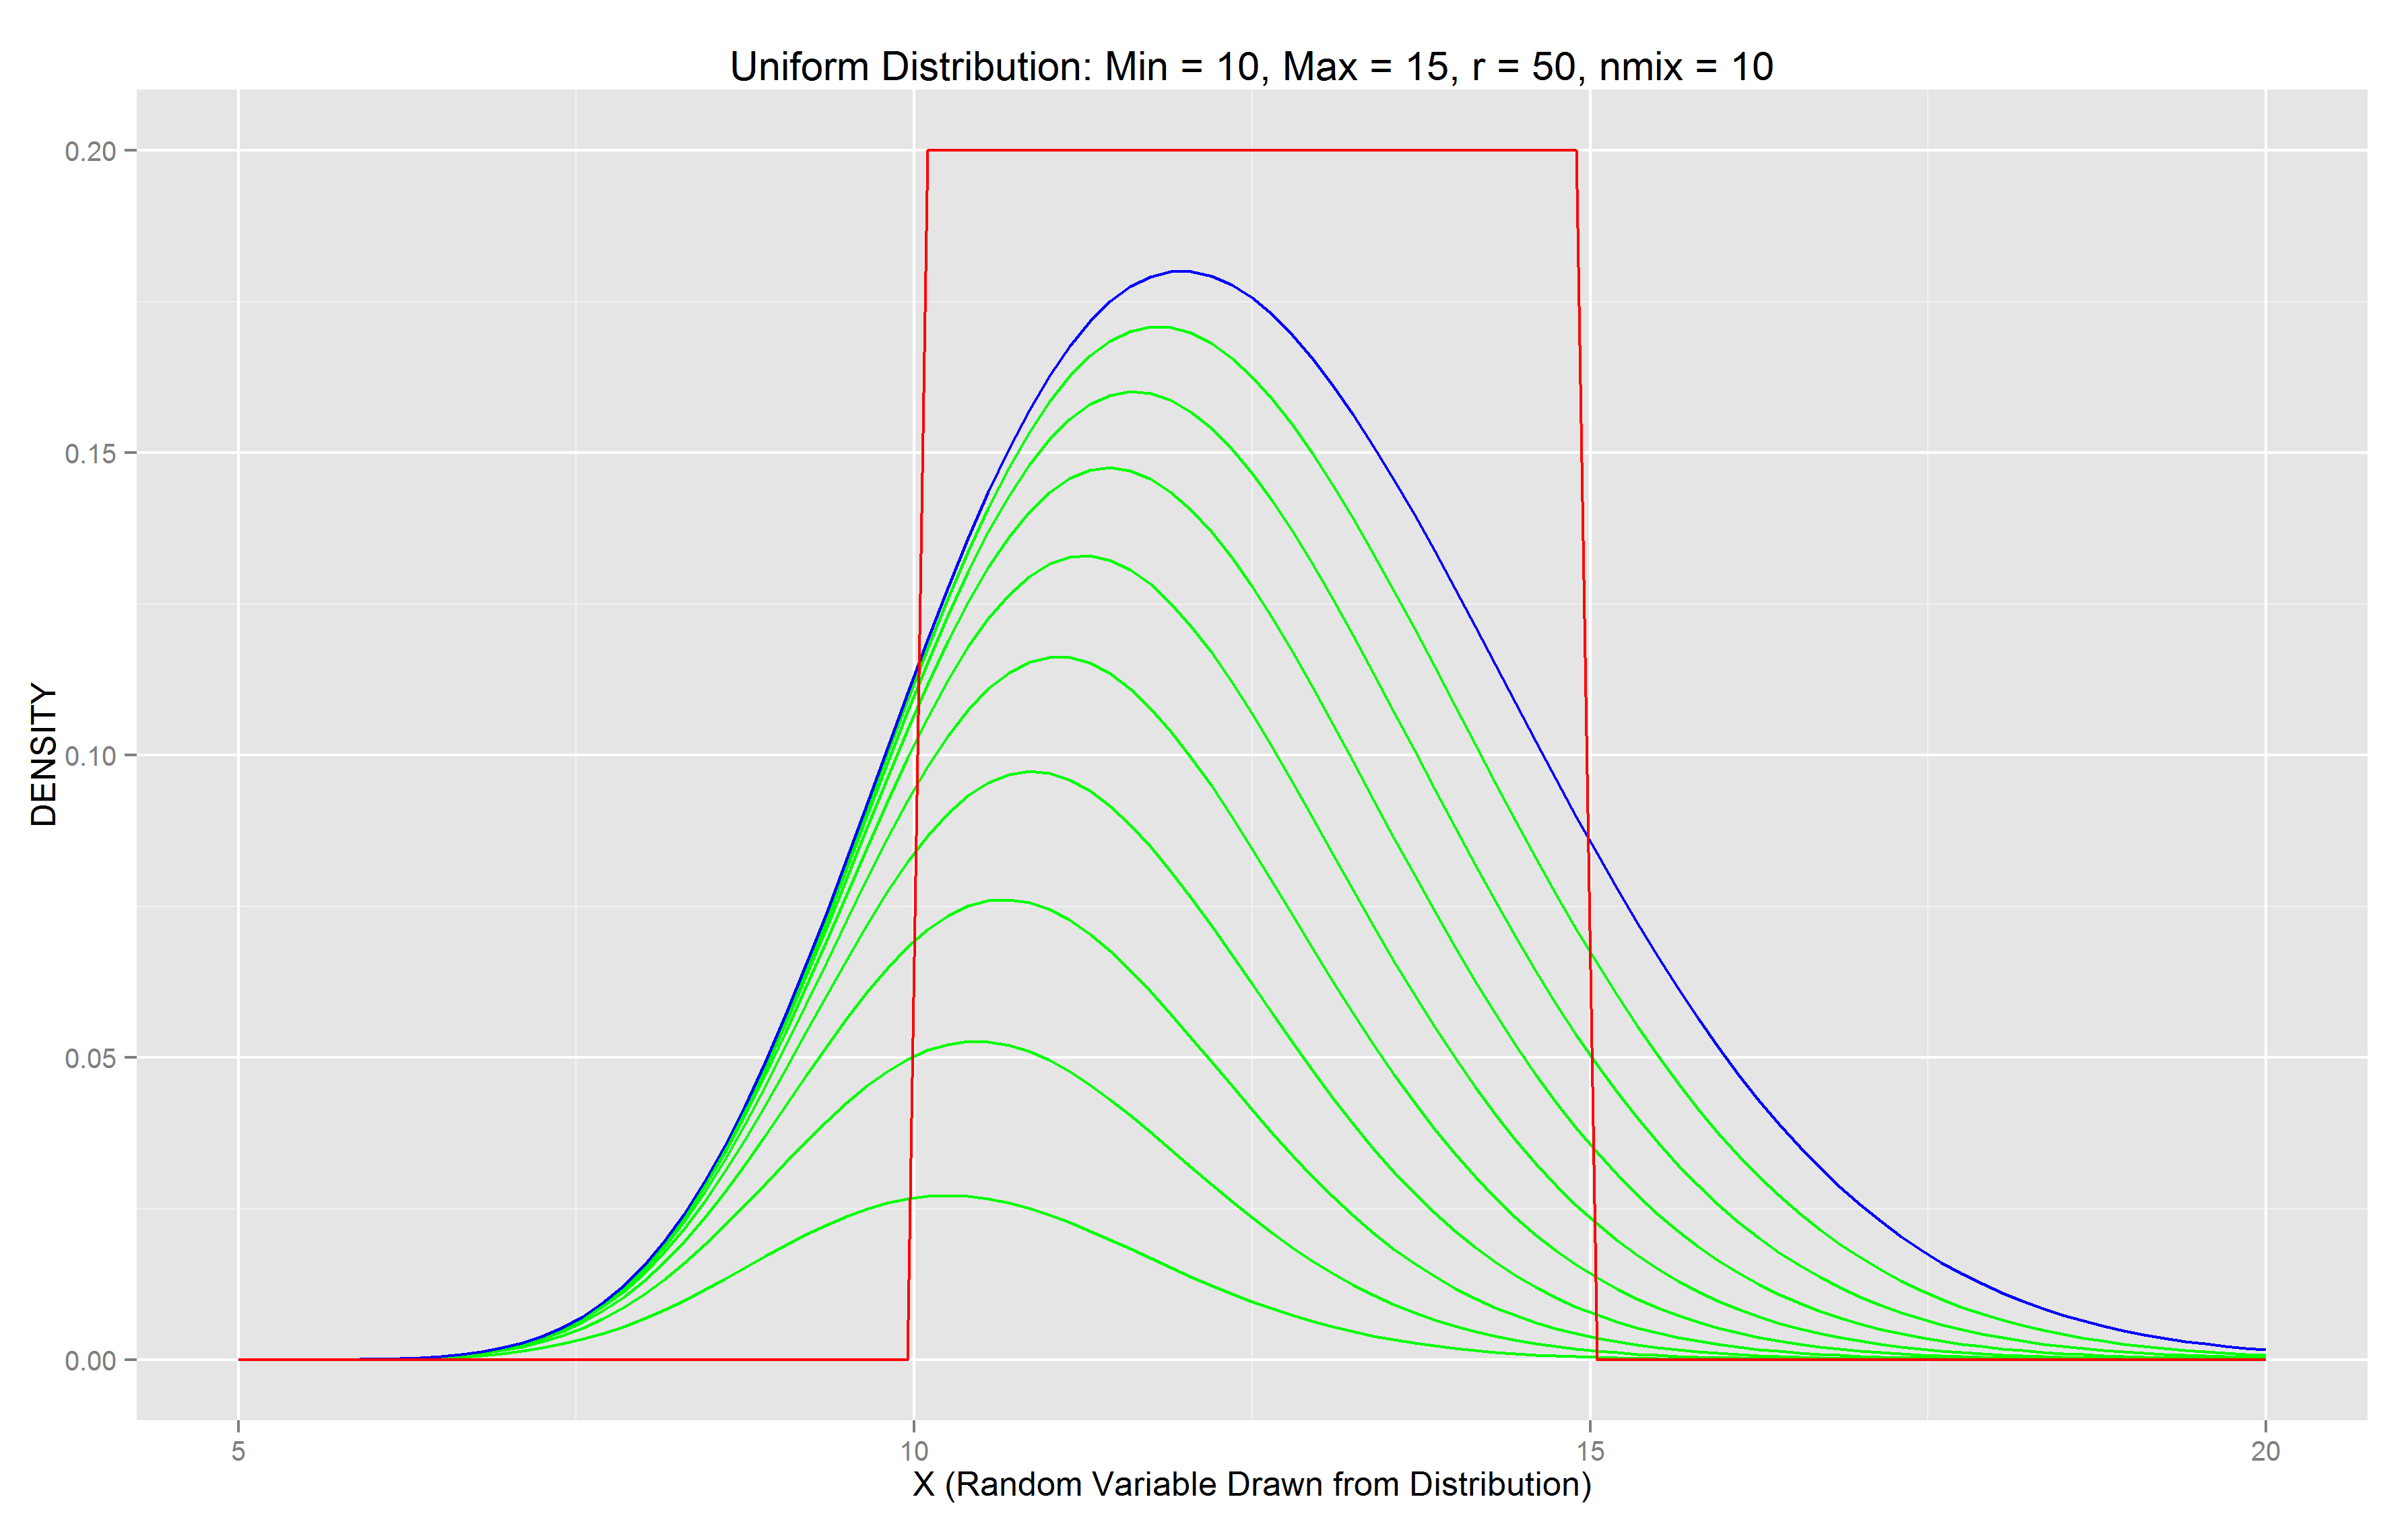
\includegraphics[scale=.27]{unifdist_10_15_50_10.png}
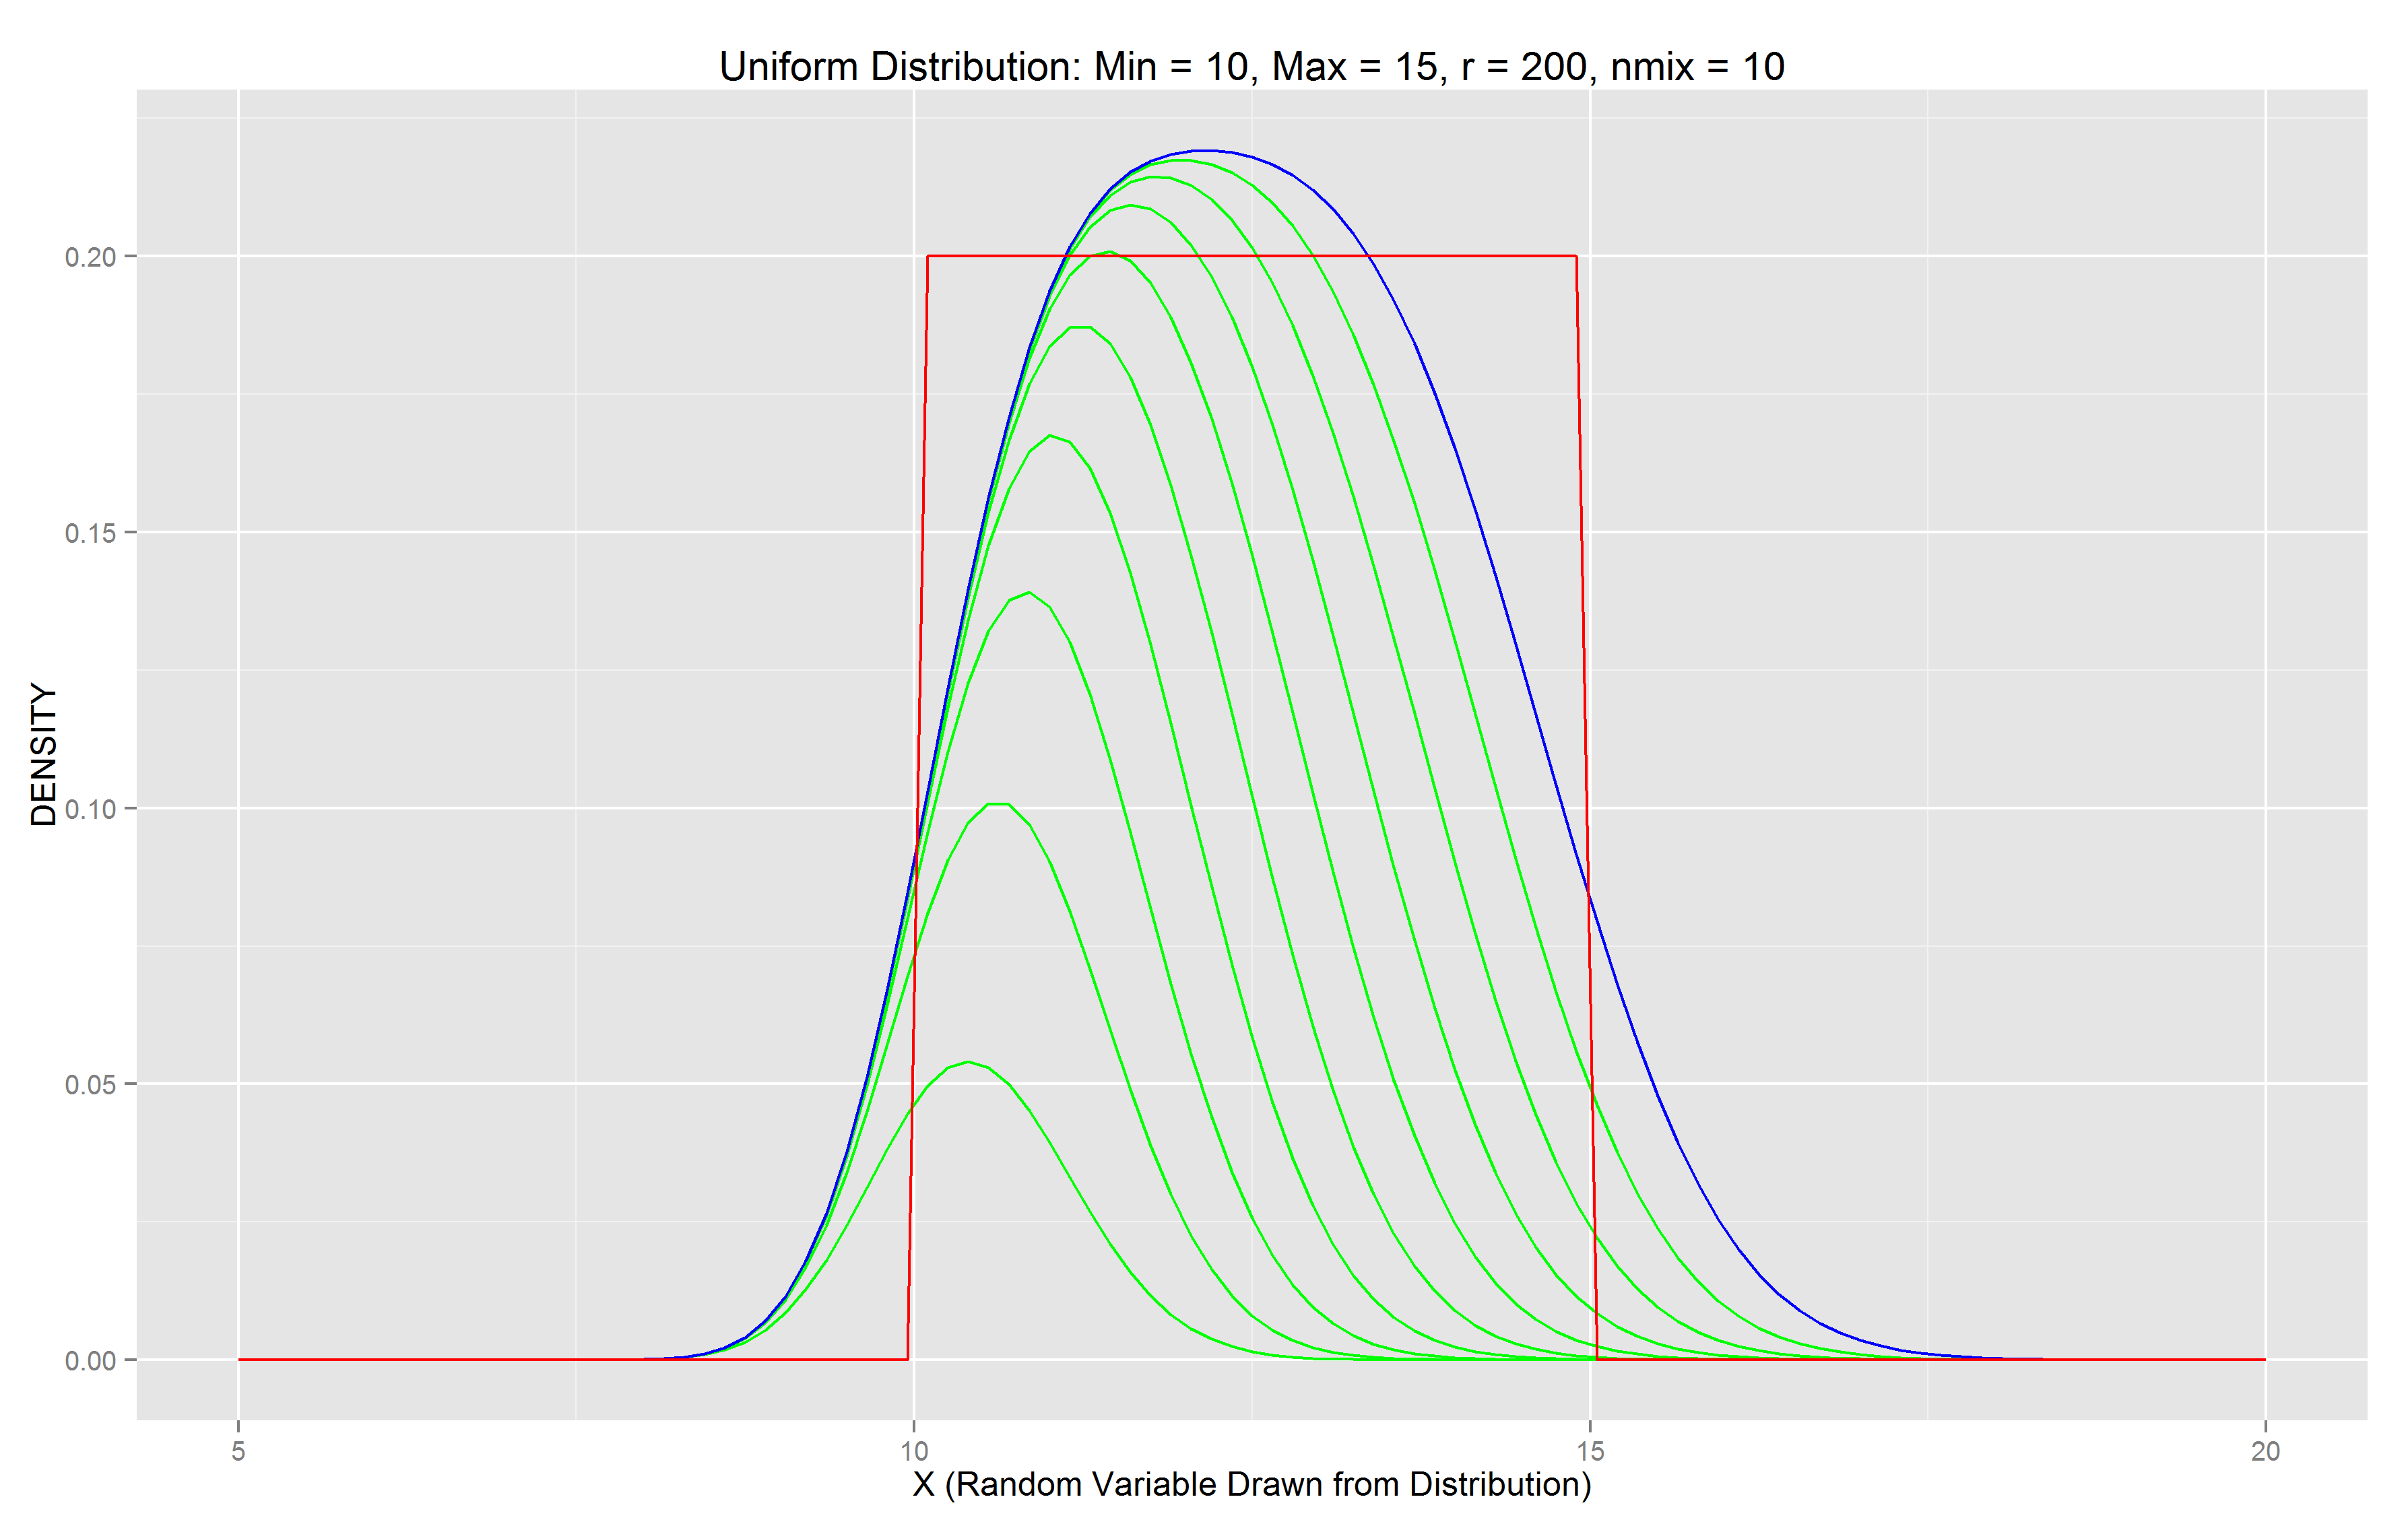
\includegraphics[scale=.27]{unifdist_10_15_200_10.png}\\
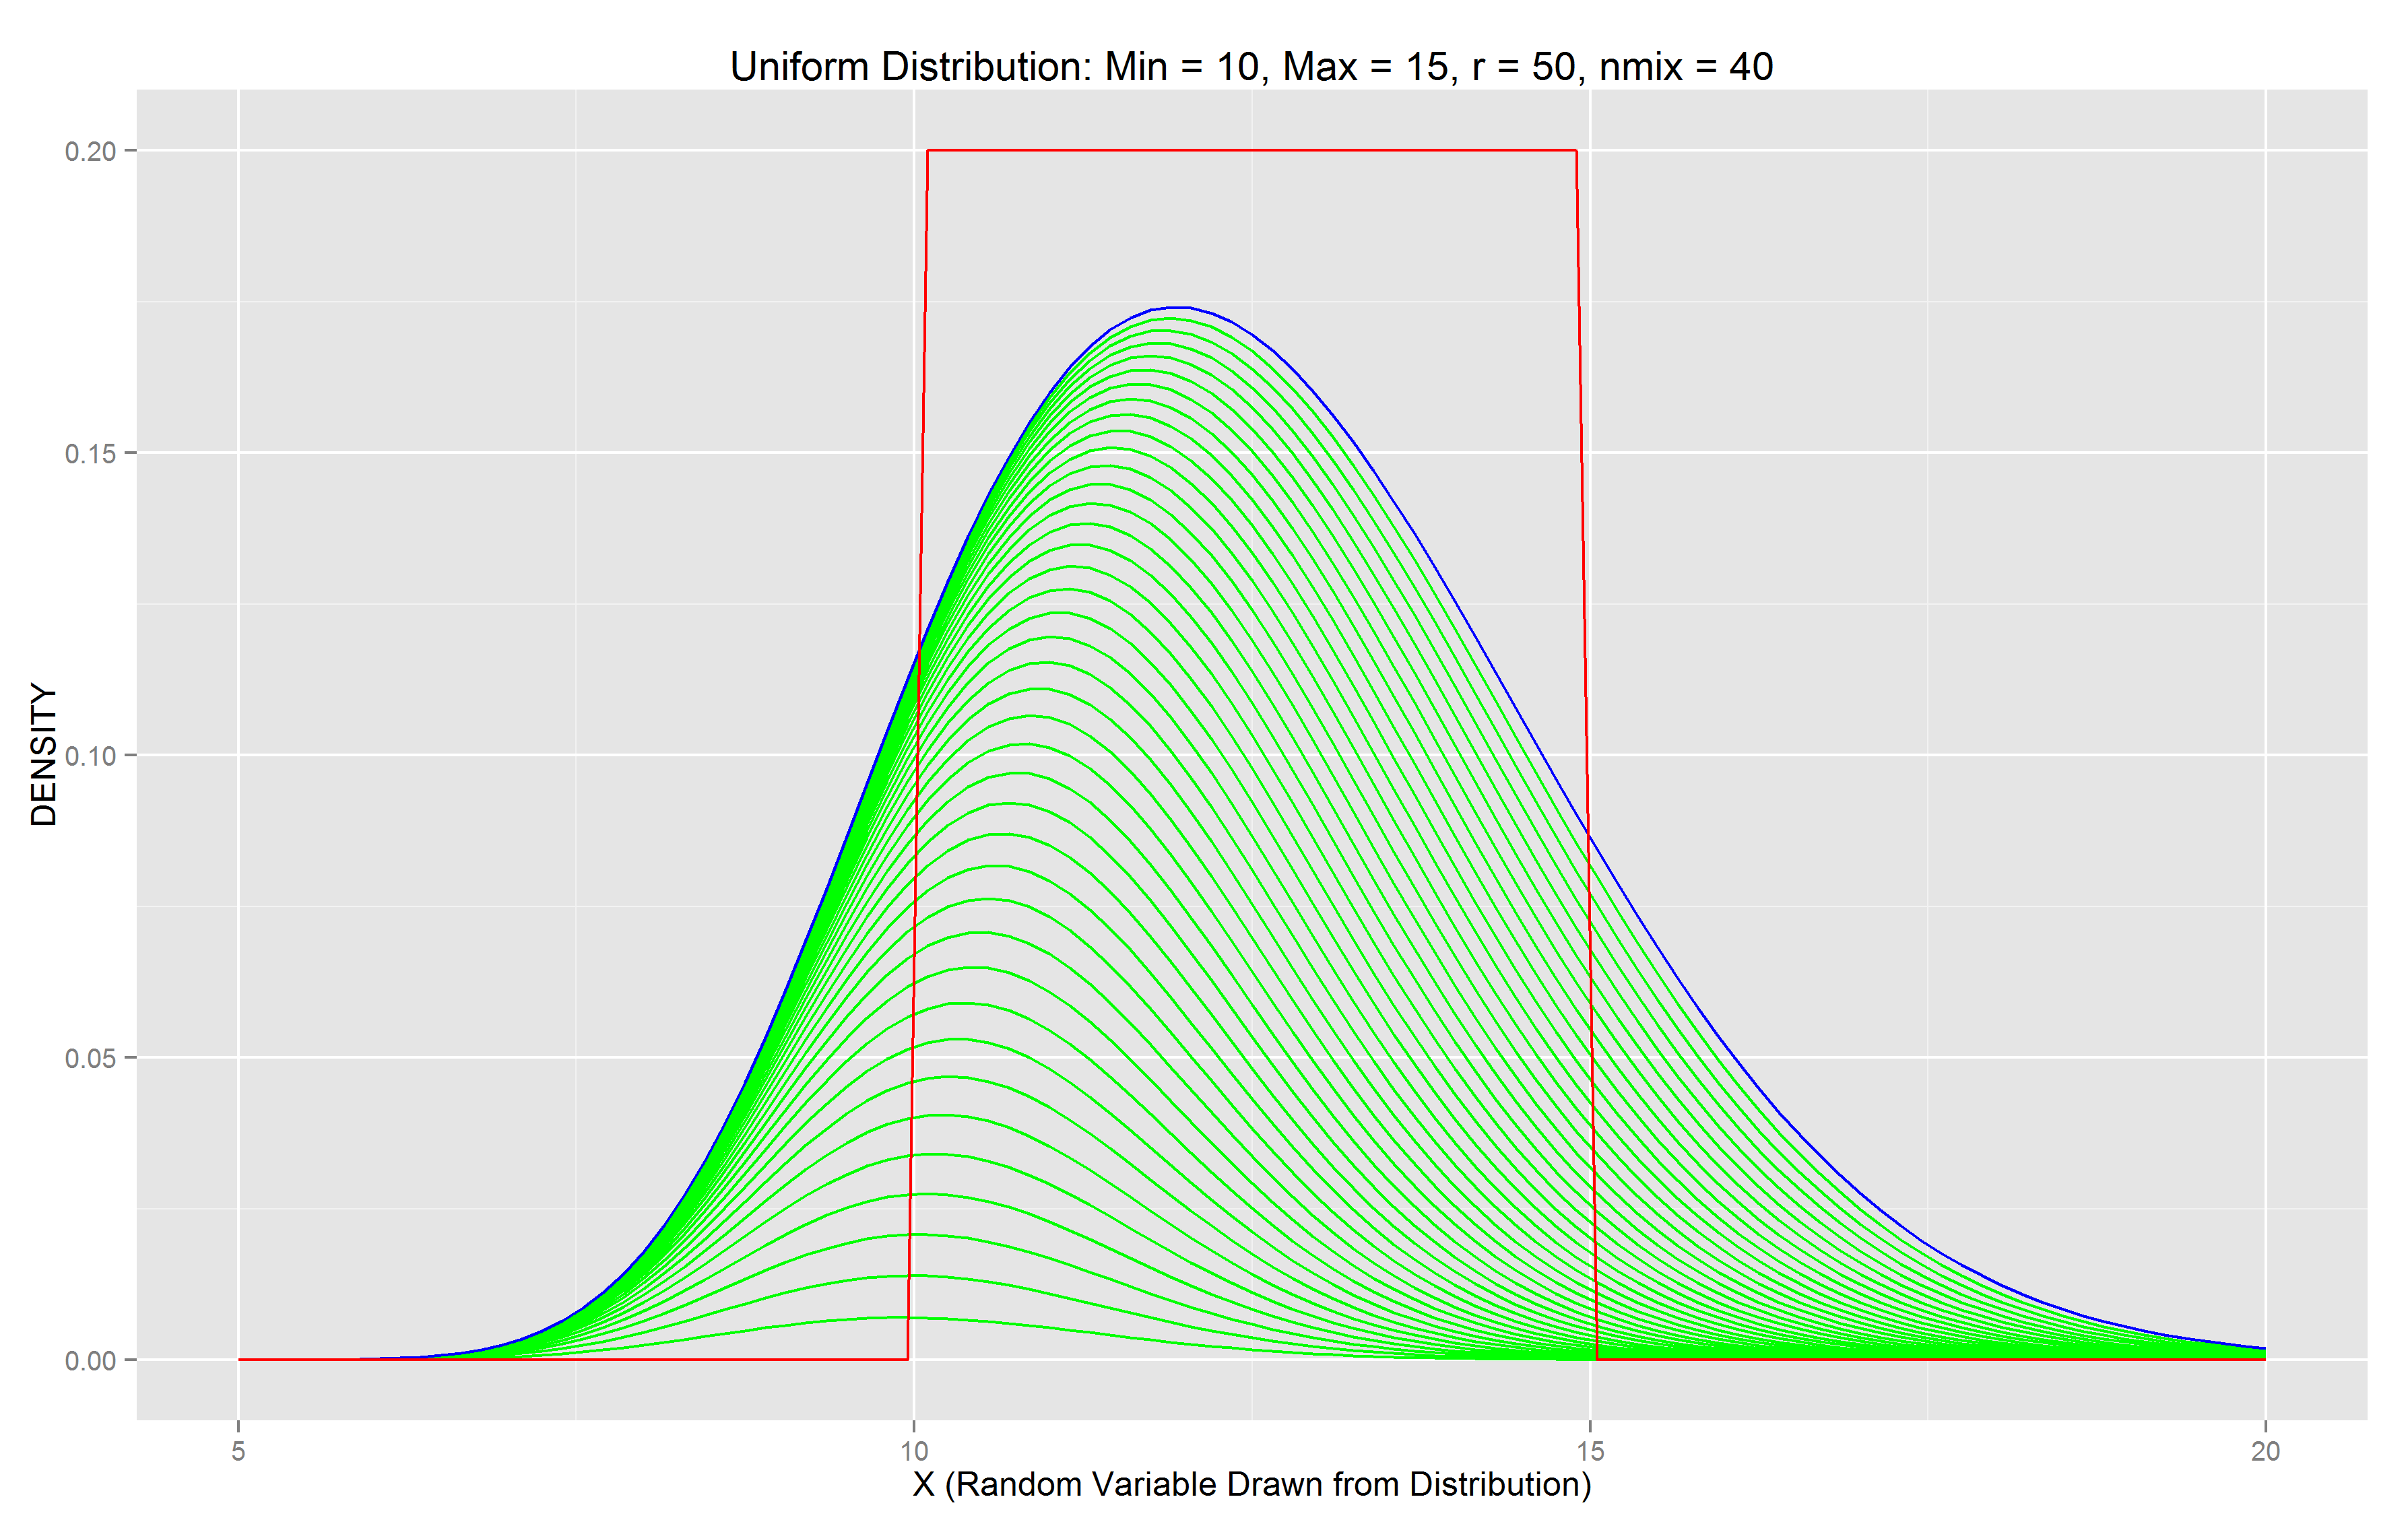
\includegraphics[scale=.27]{unifdist_10_15_50_40.png}
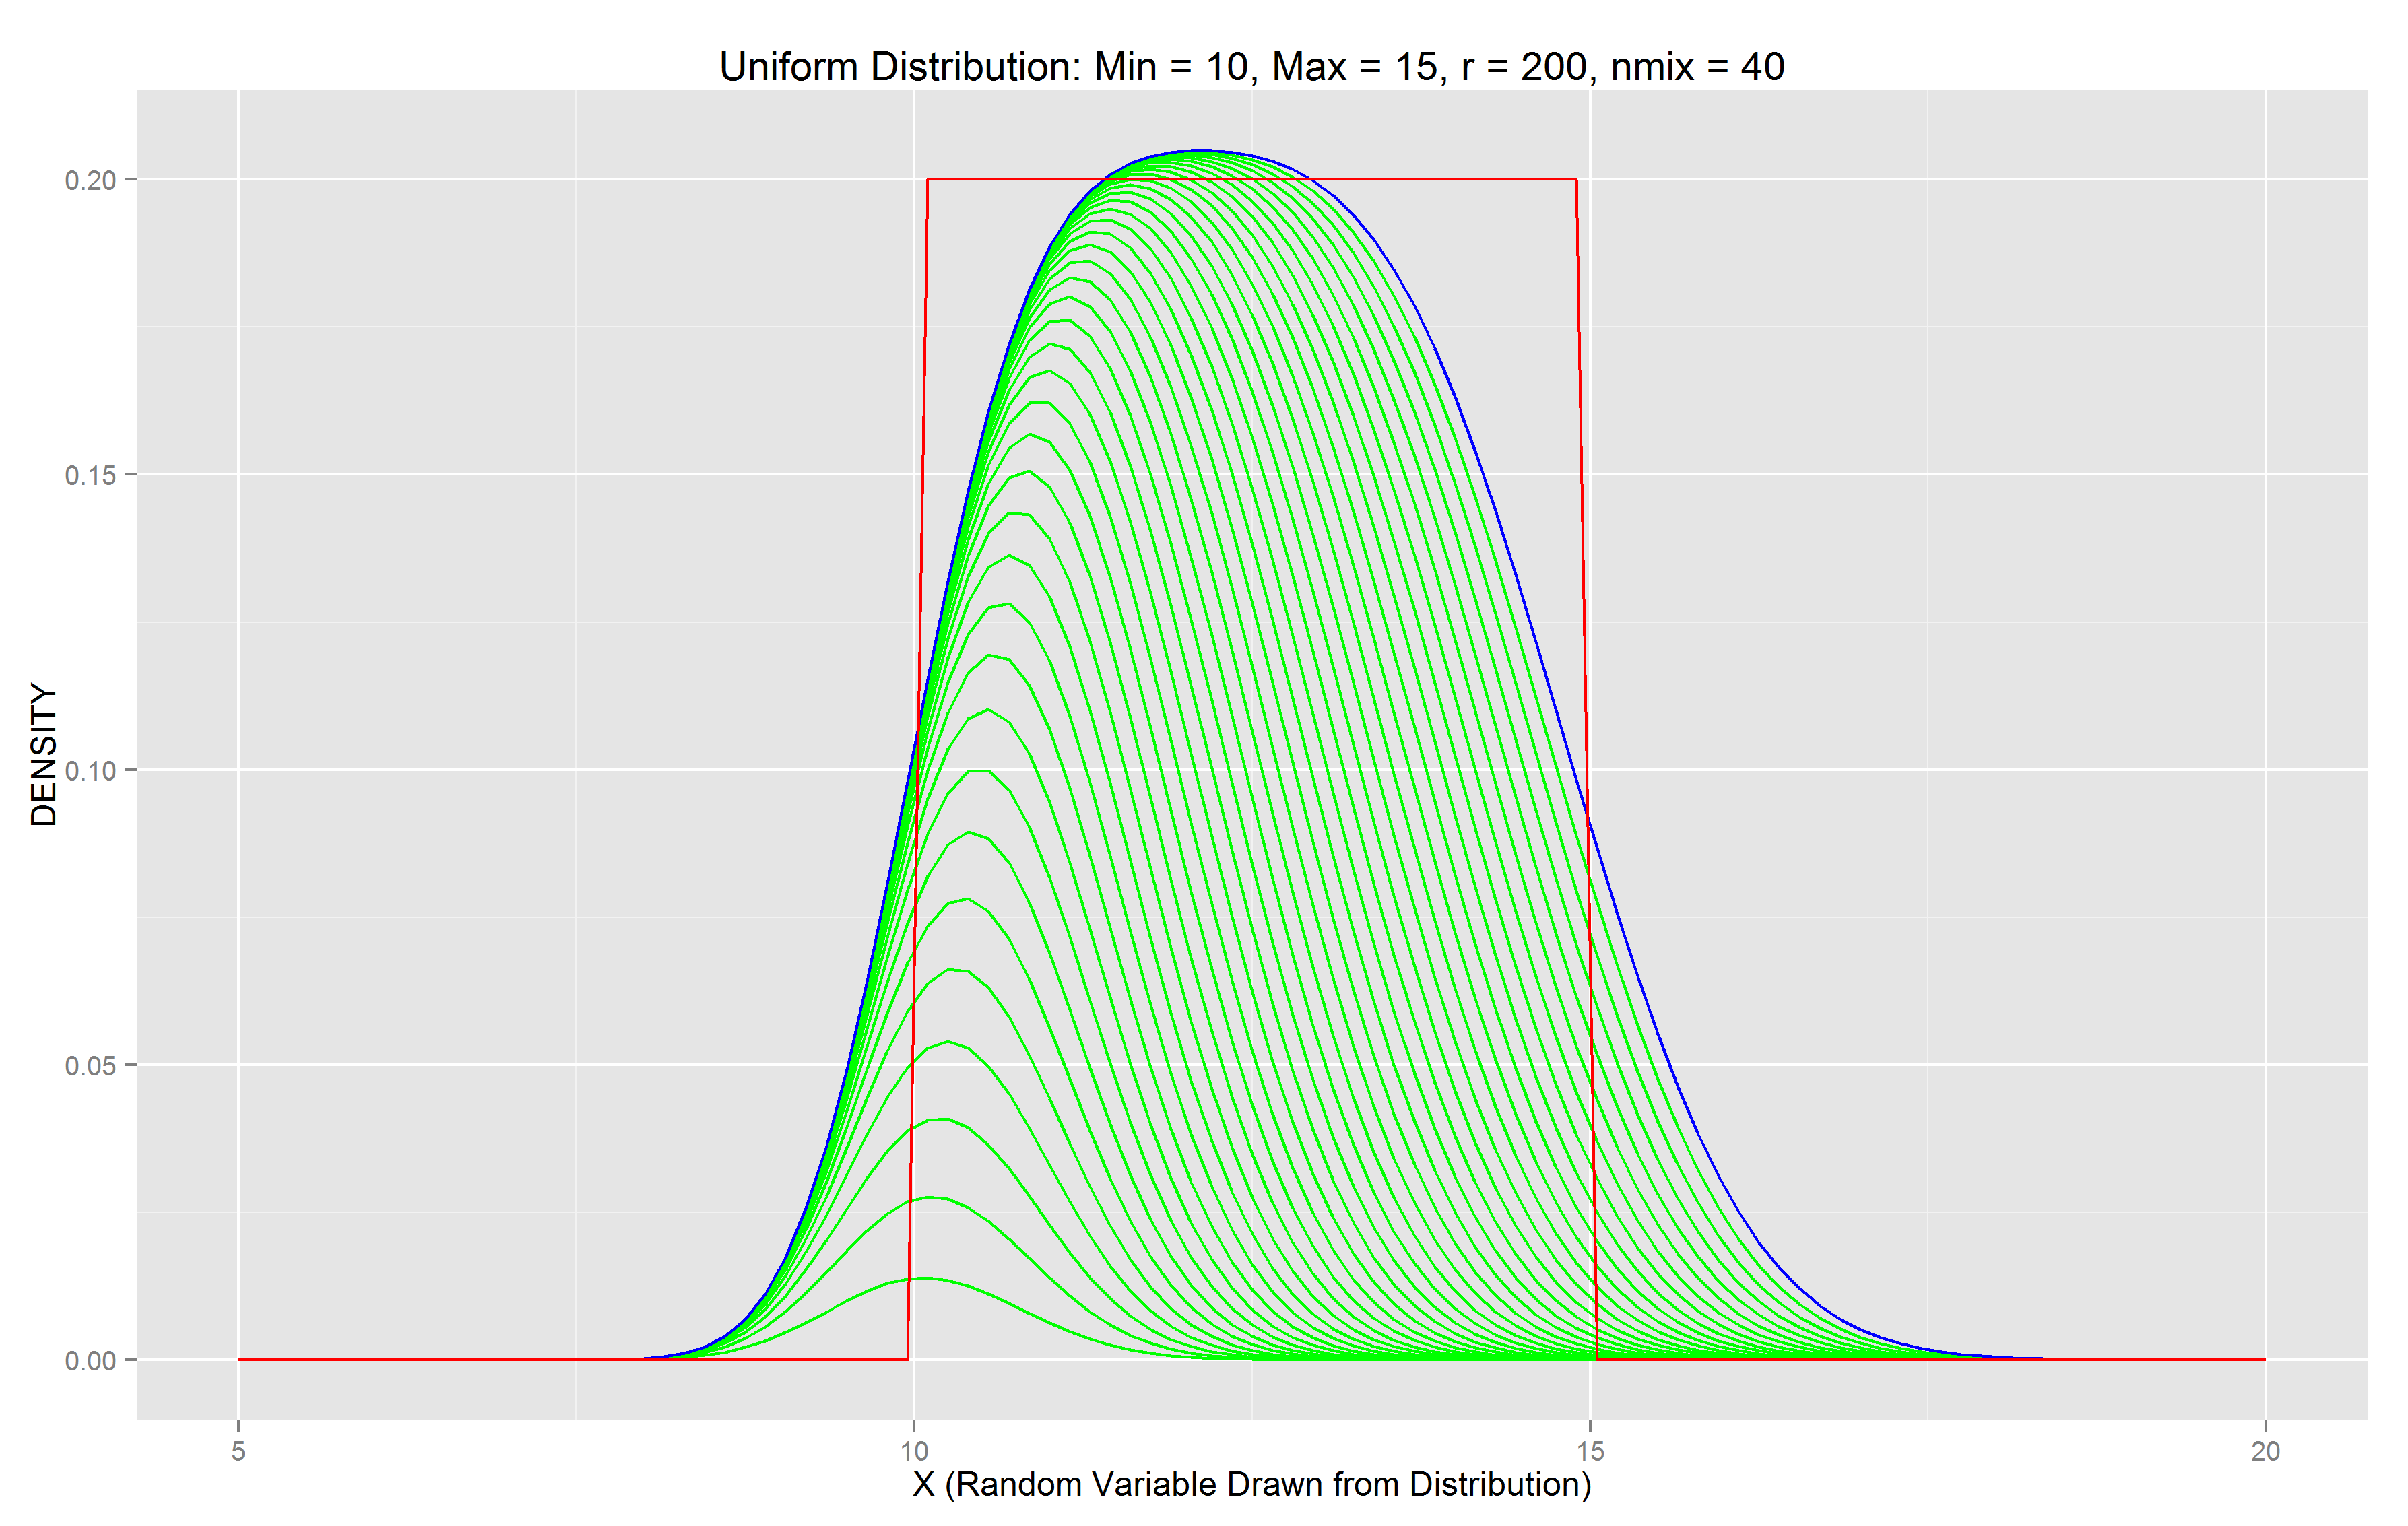
\includegraphics[scale=.27]{unifdist_10_15_200_40.png}\\
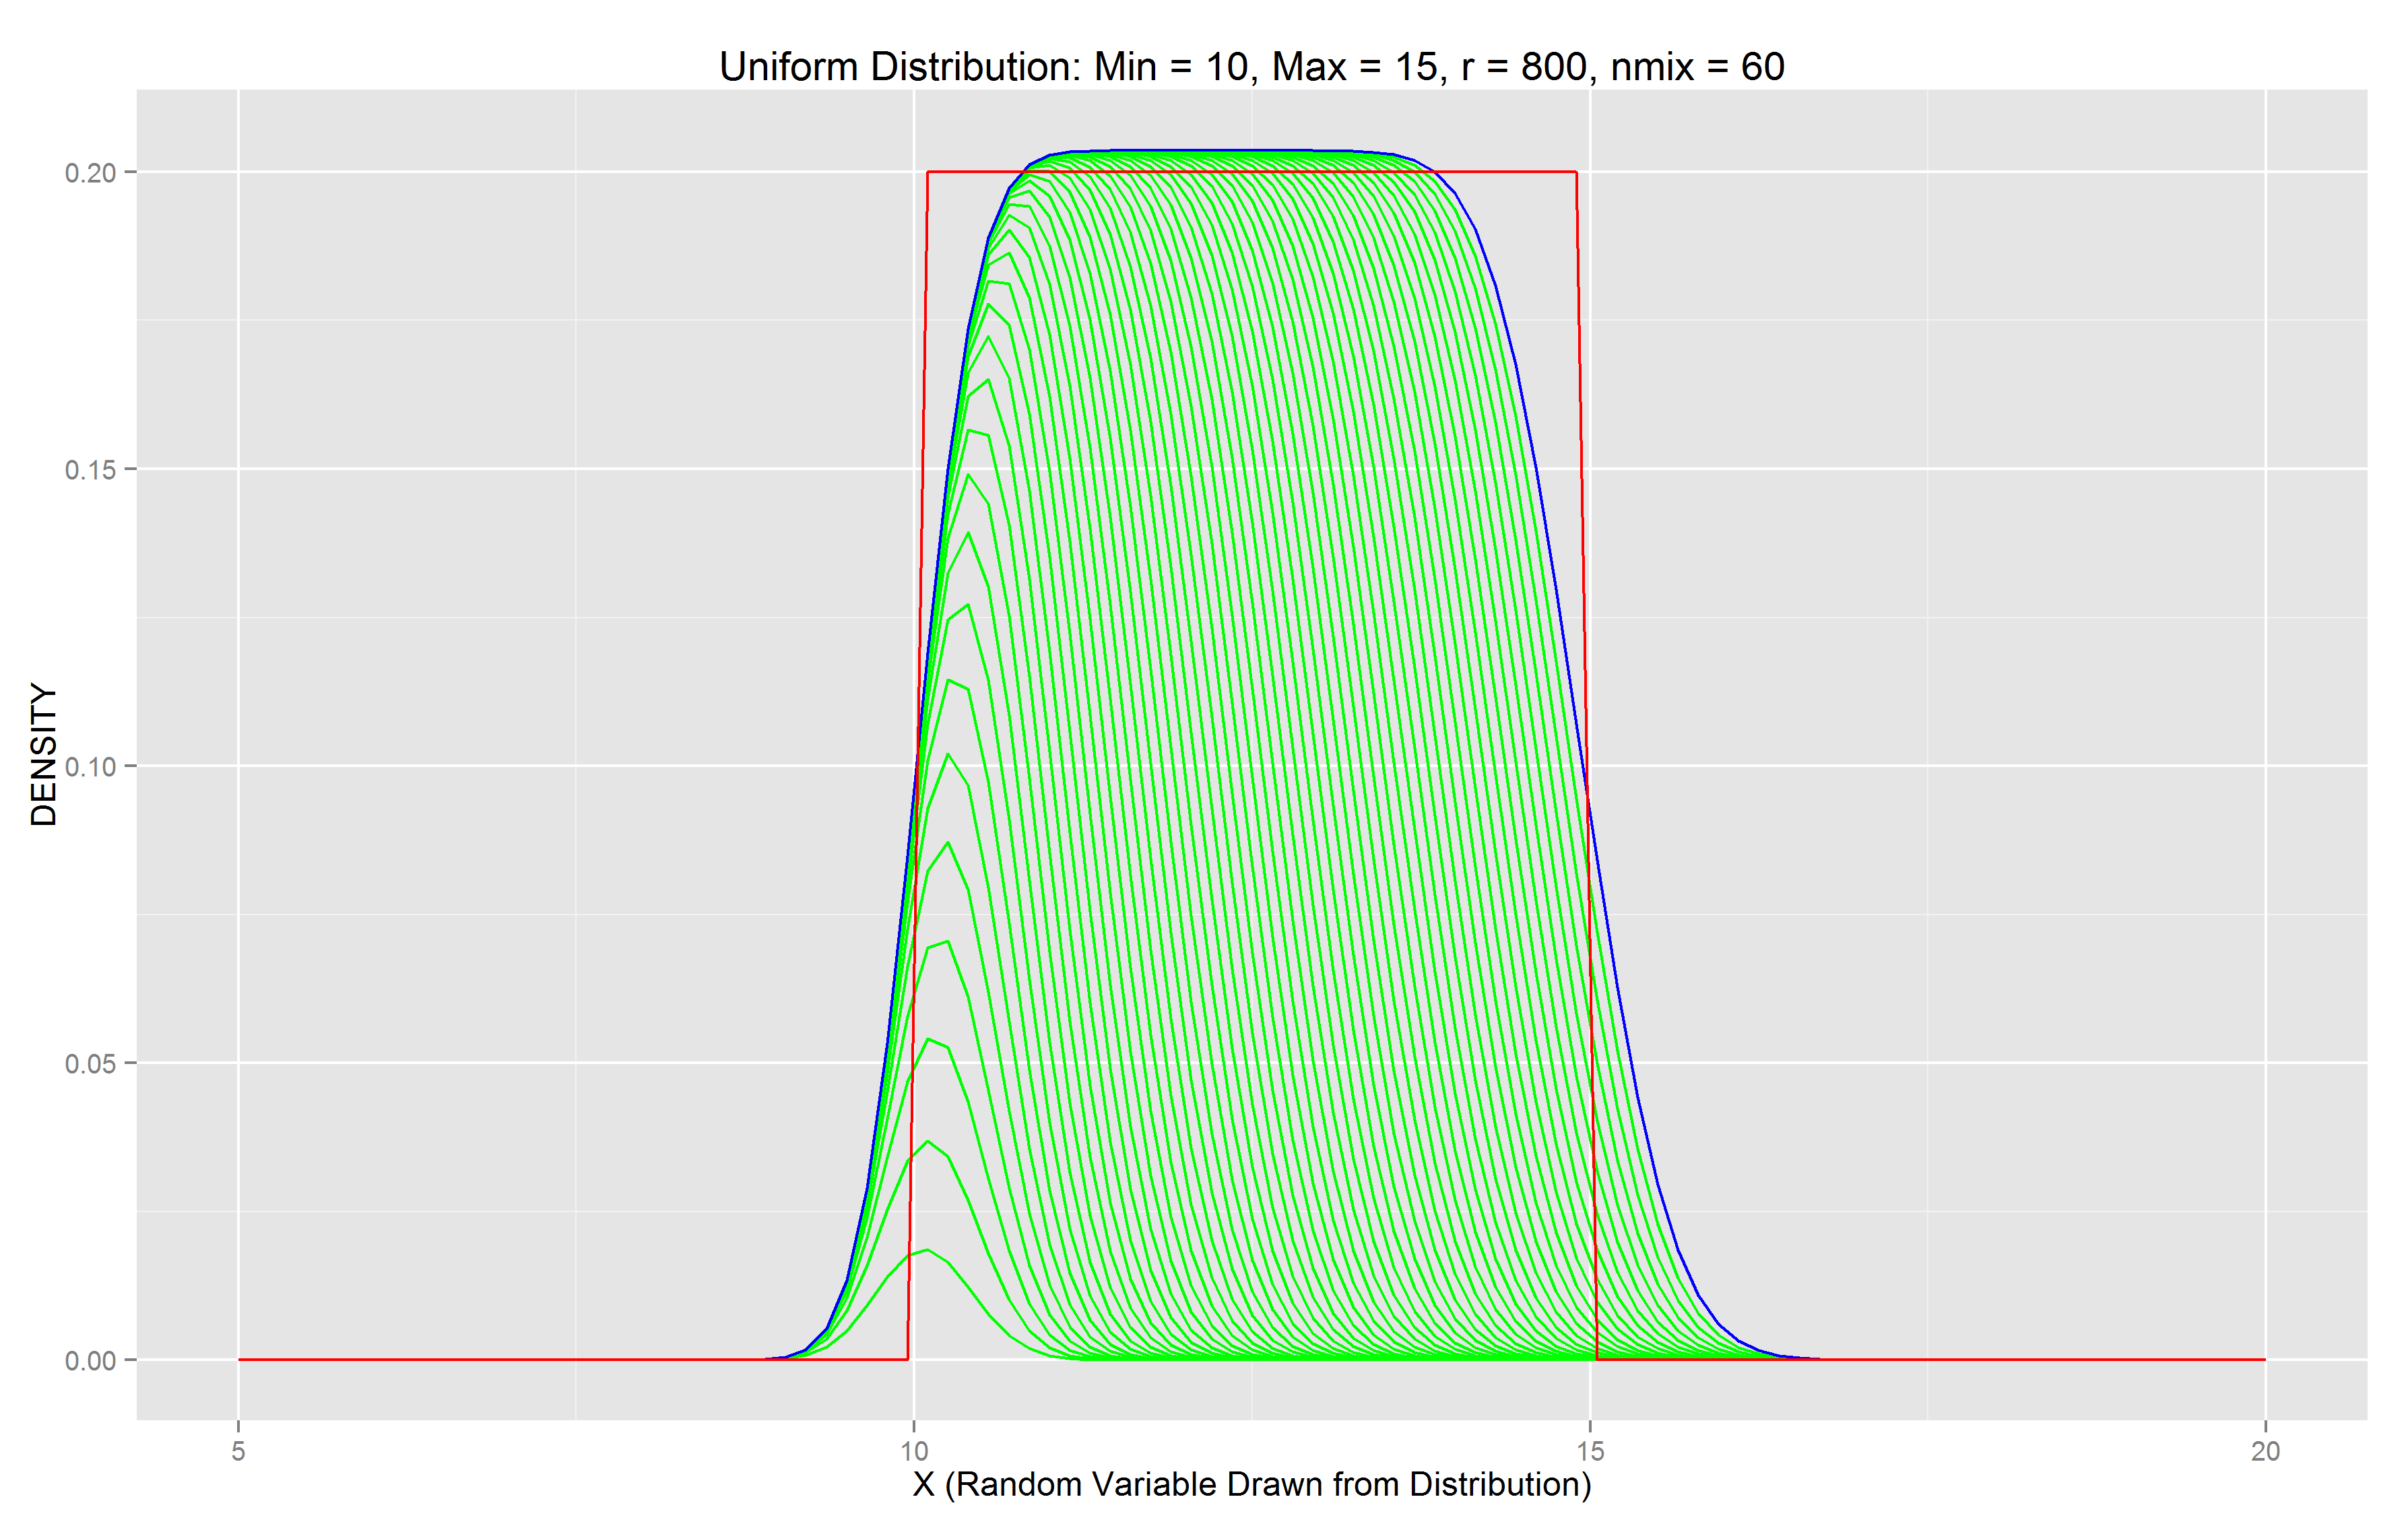
\includegraphics[scale=.54]{unifdist_10_15_800_60.png}
\end{figure}


\begin{figure}[H]
\centering
\newpage
\Large{For a normal distribution with mean = 10, standard deviation = 4:}\\
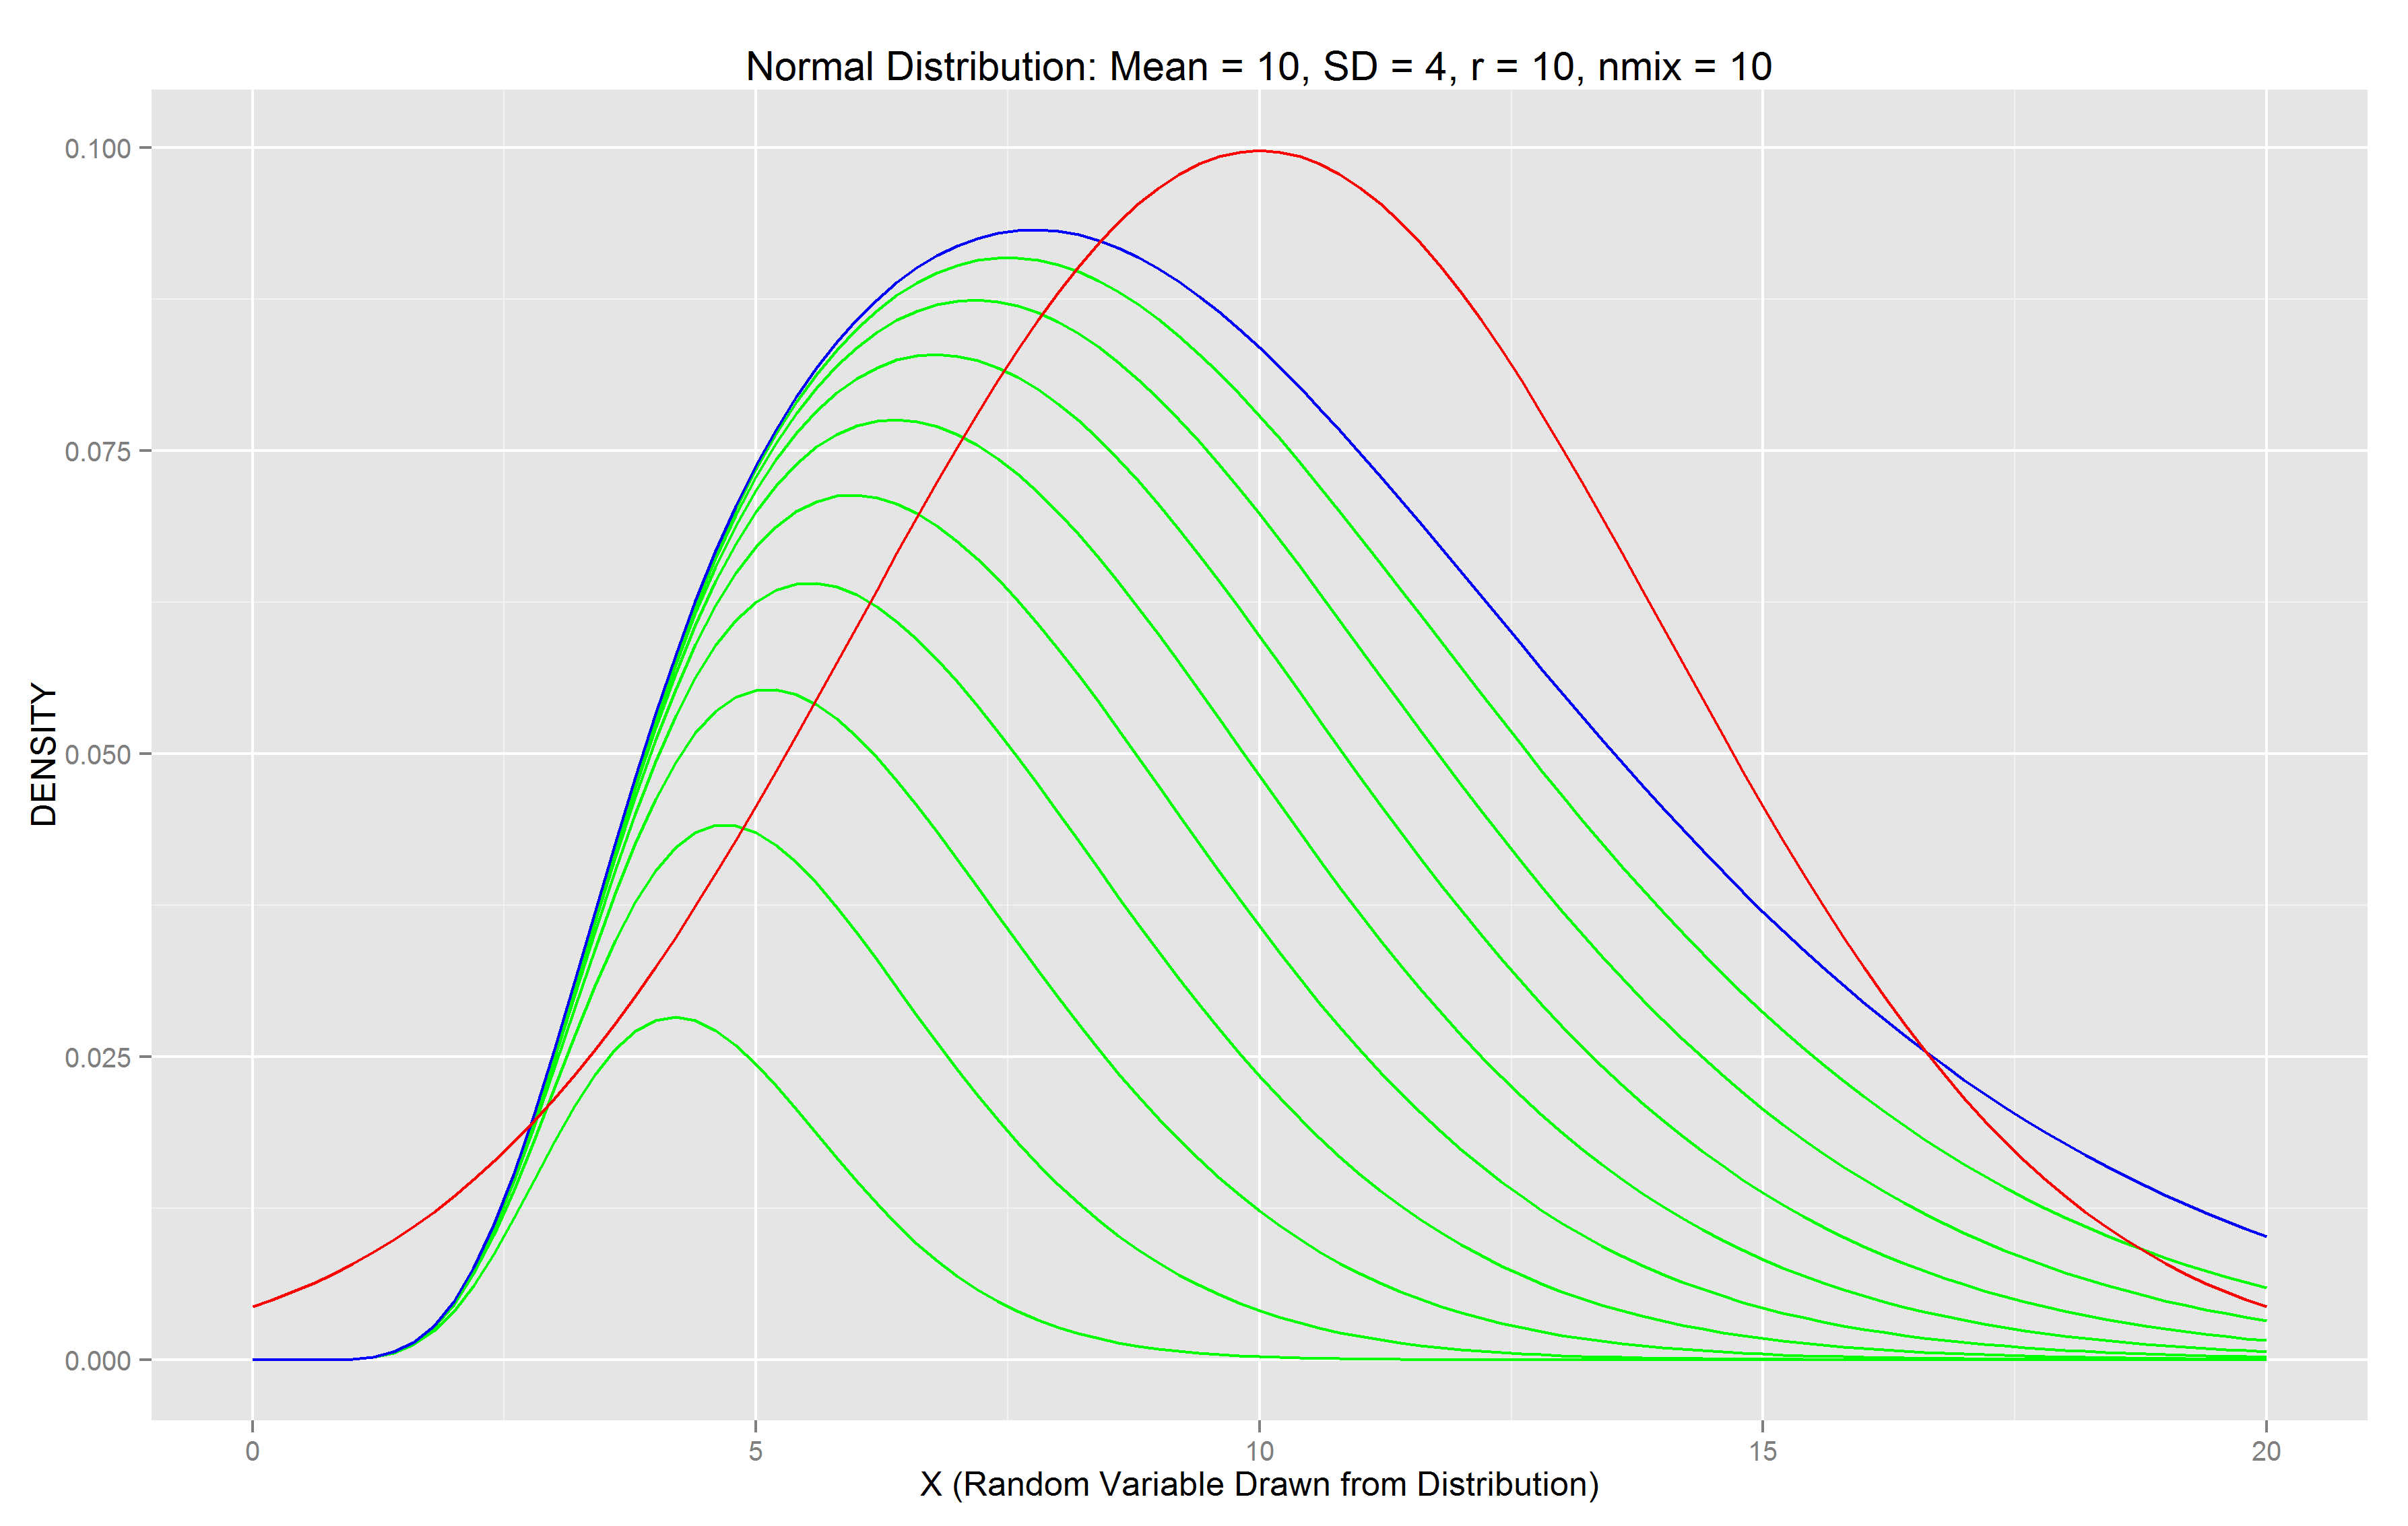
\includegraphics[scale=.27]{normdist_10_4_10_10.png}
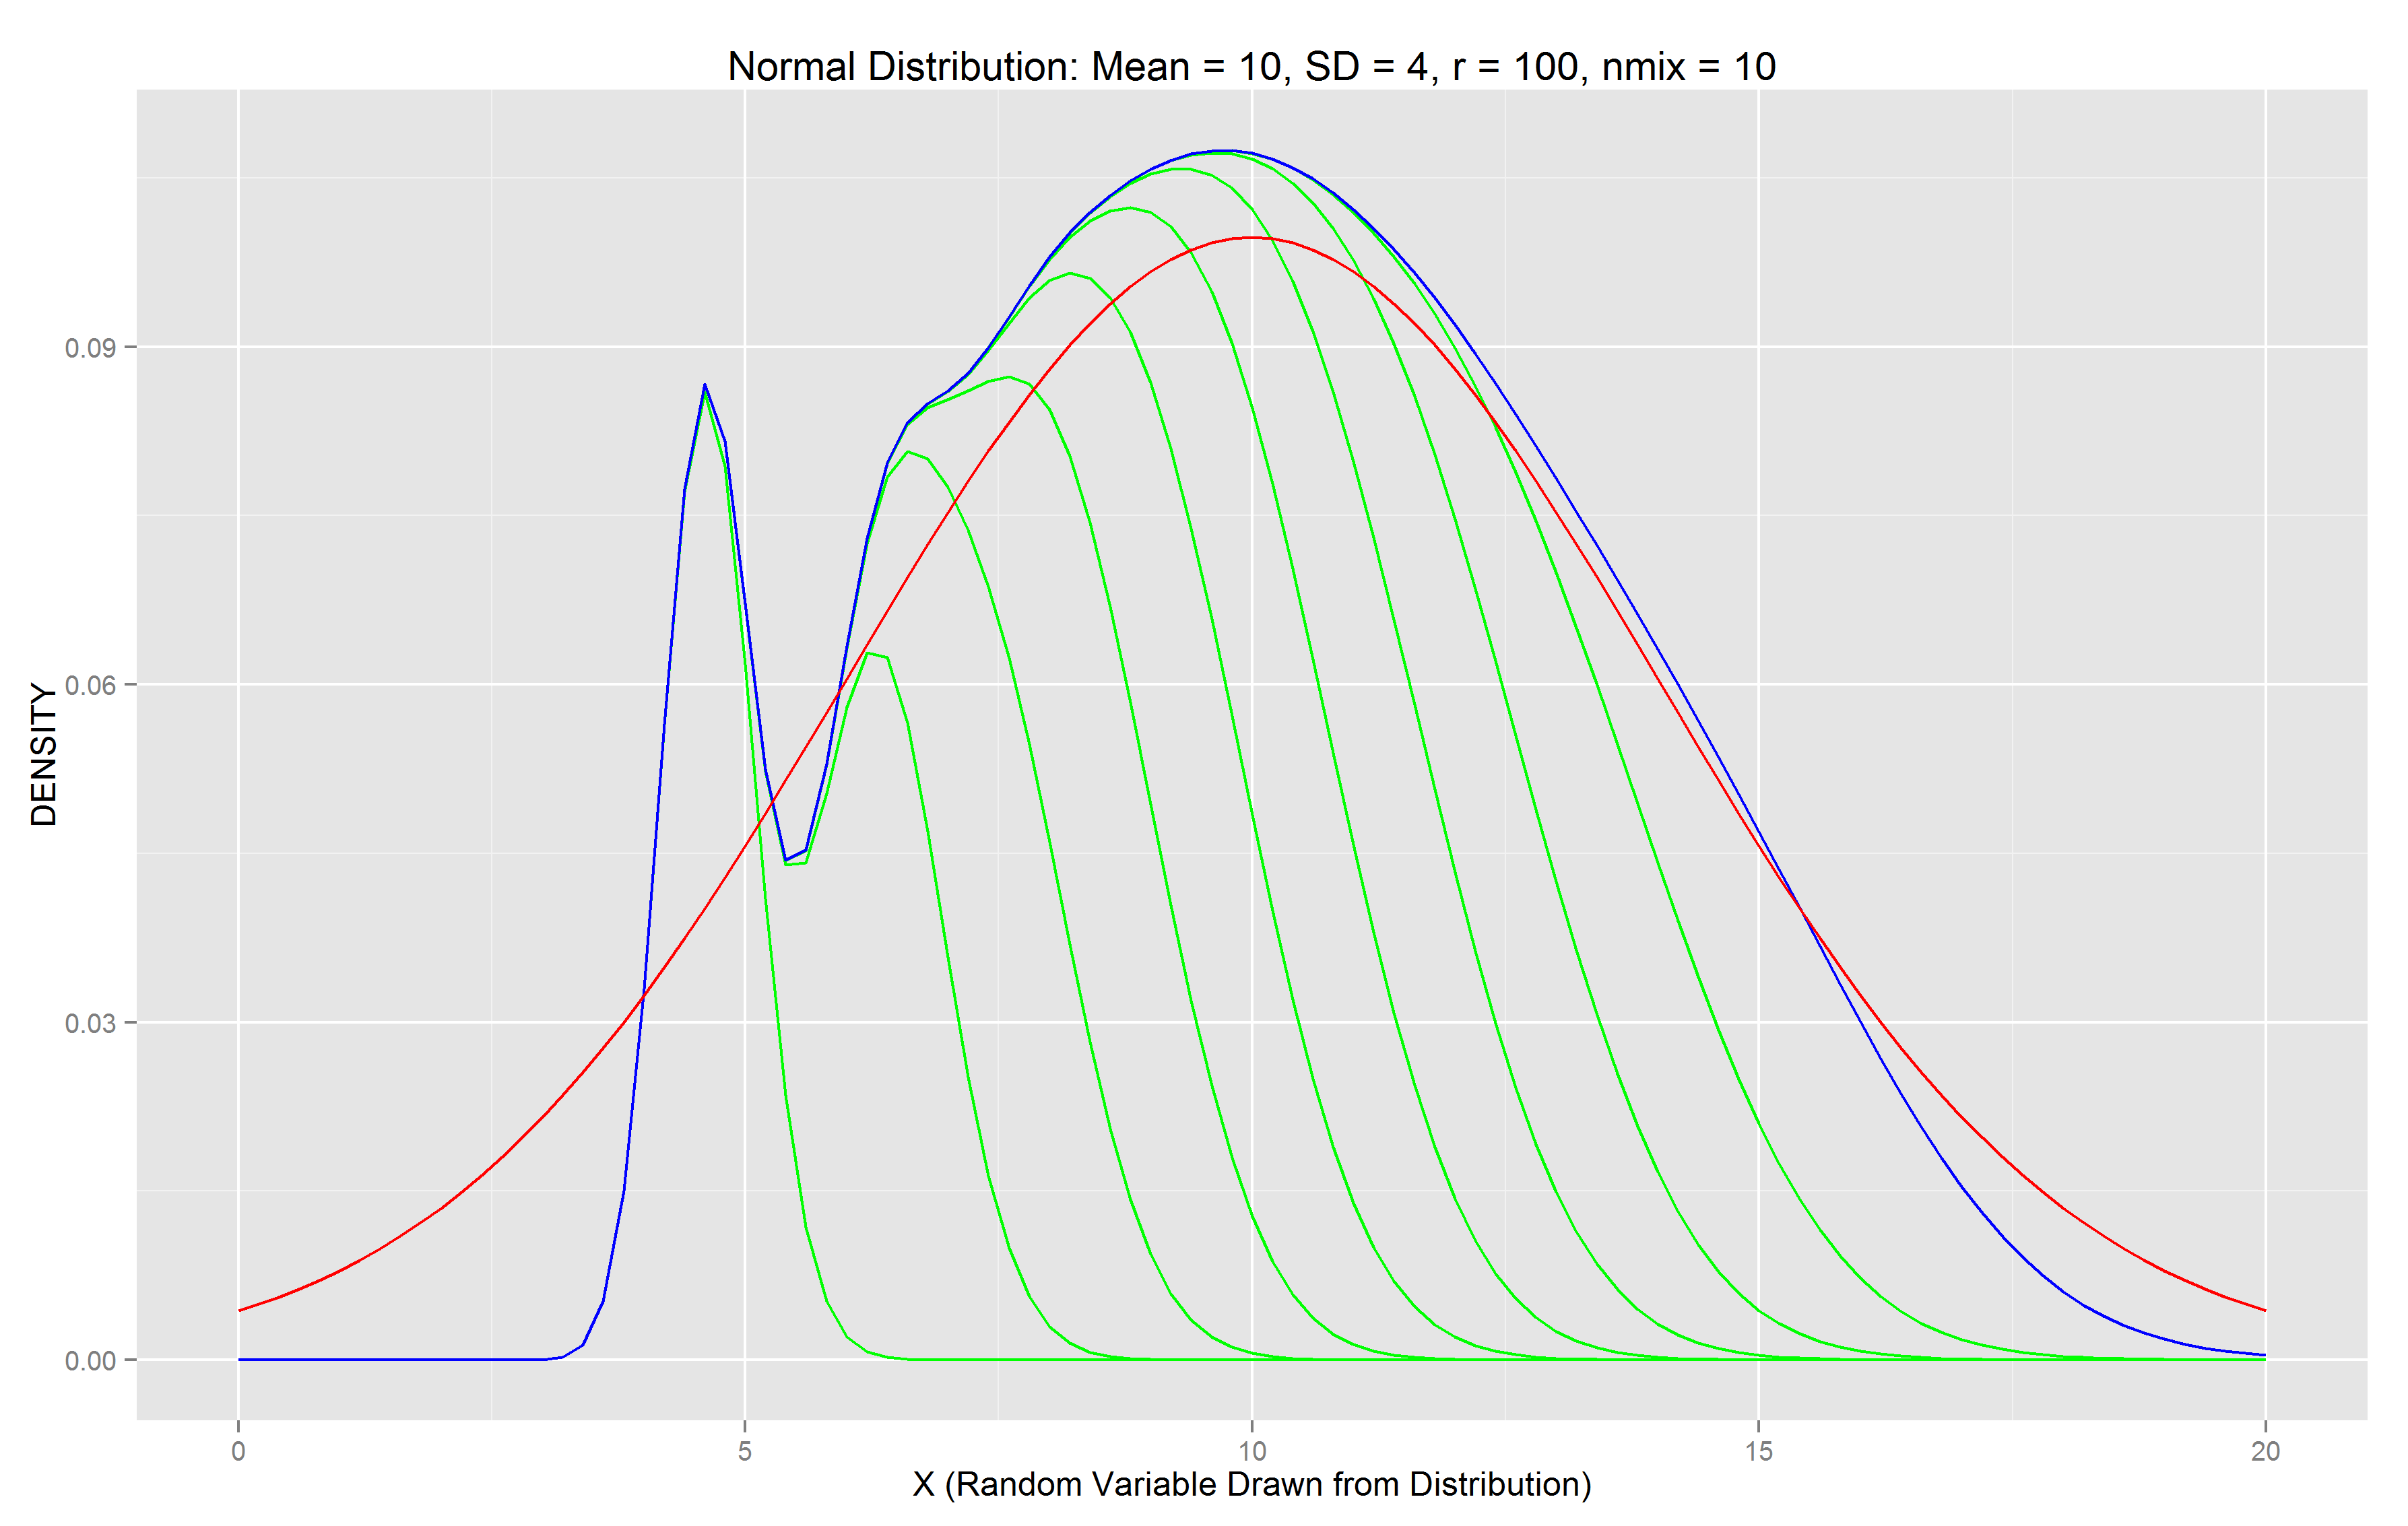
\includegraphics[scale=.27]{normdist_10_4_100_10.png}\\
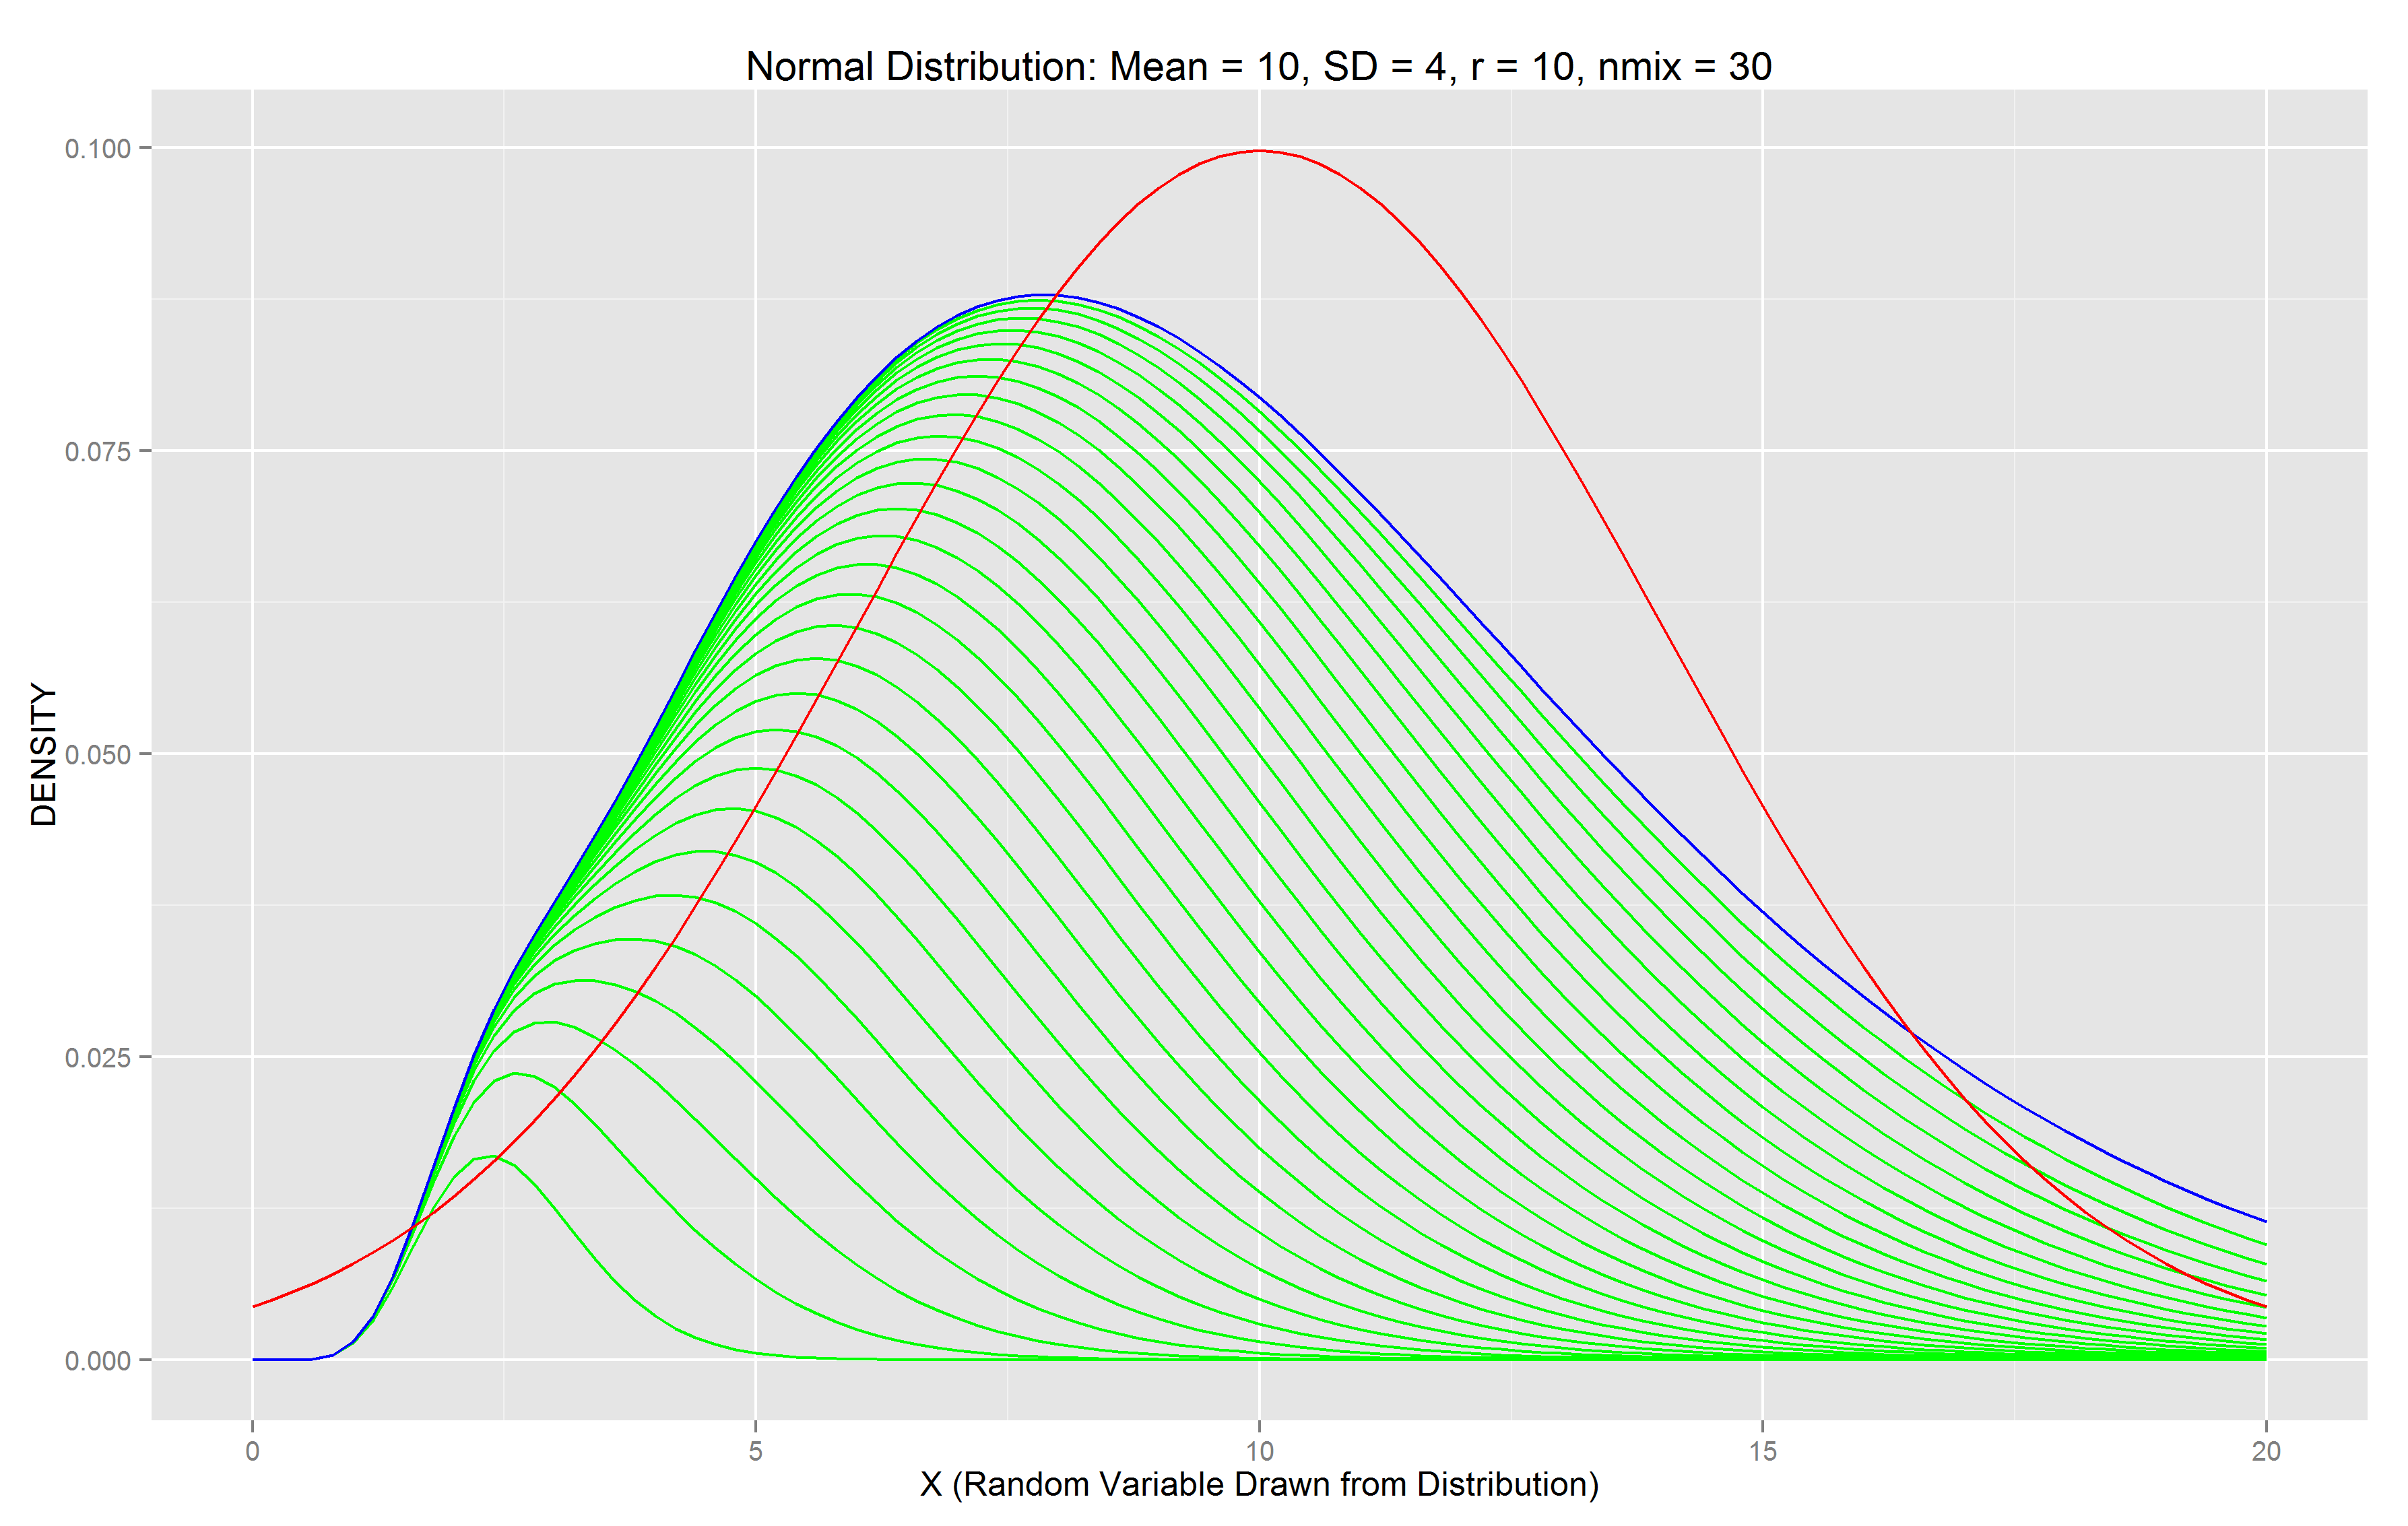
\includegraphics[scale=.27]{normdist_10_4_10_30.png}
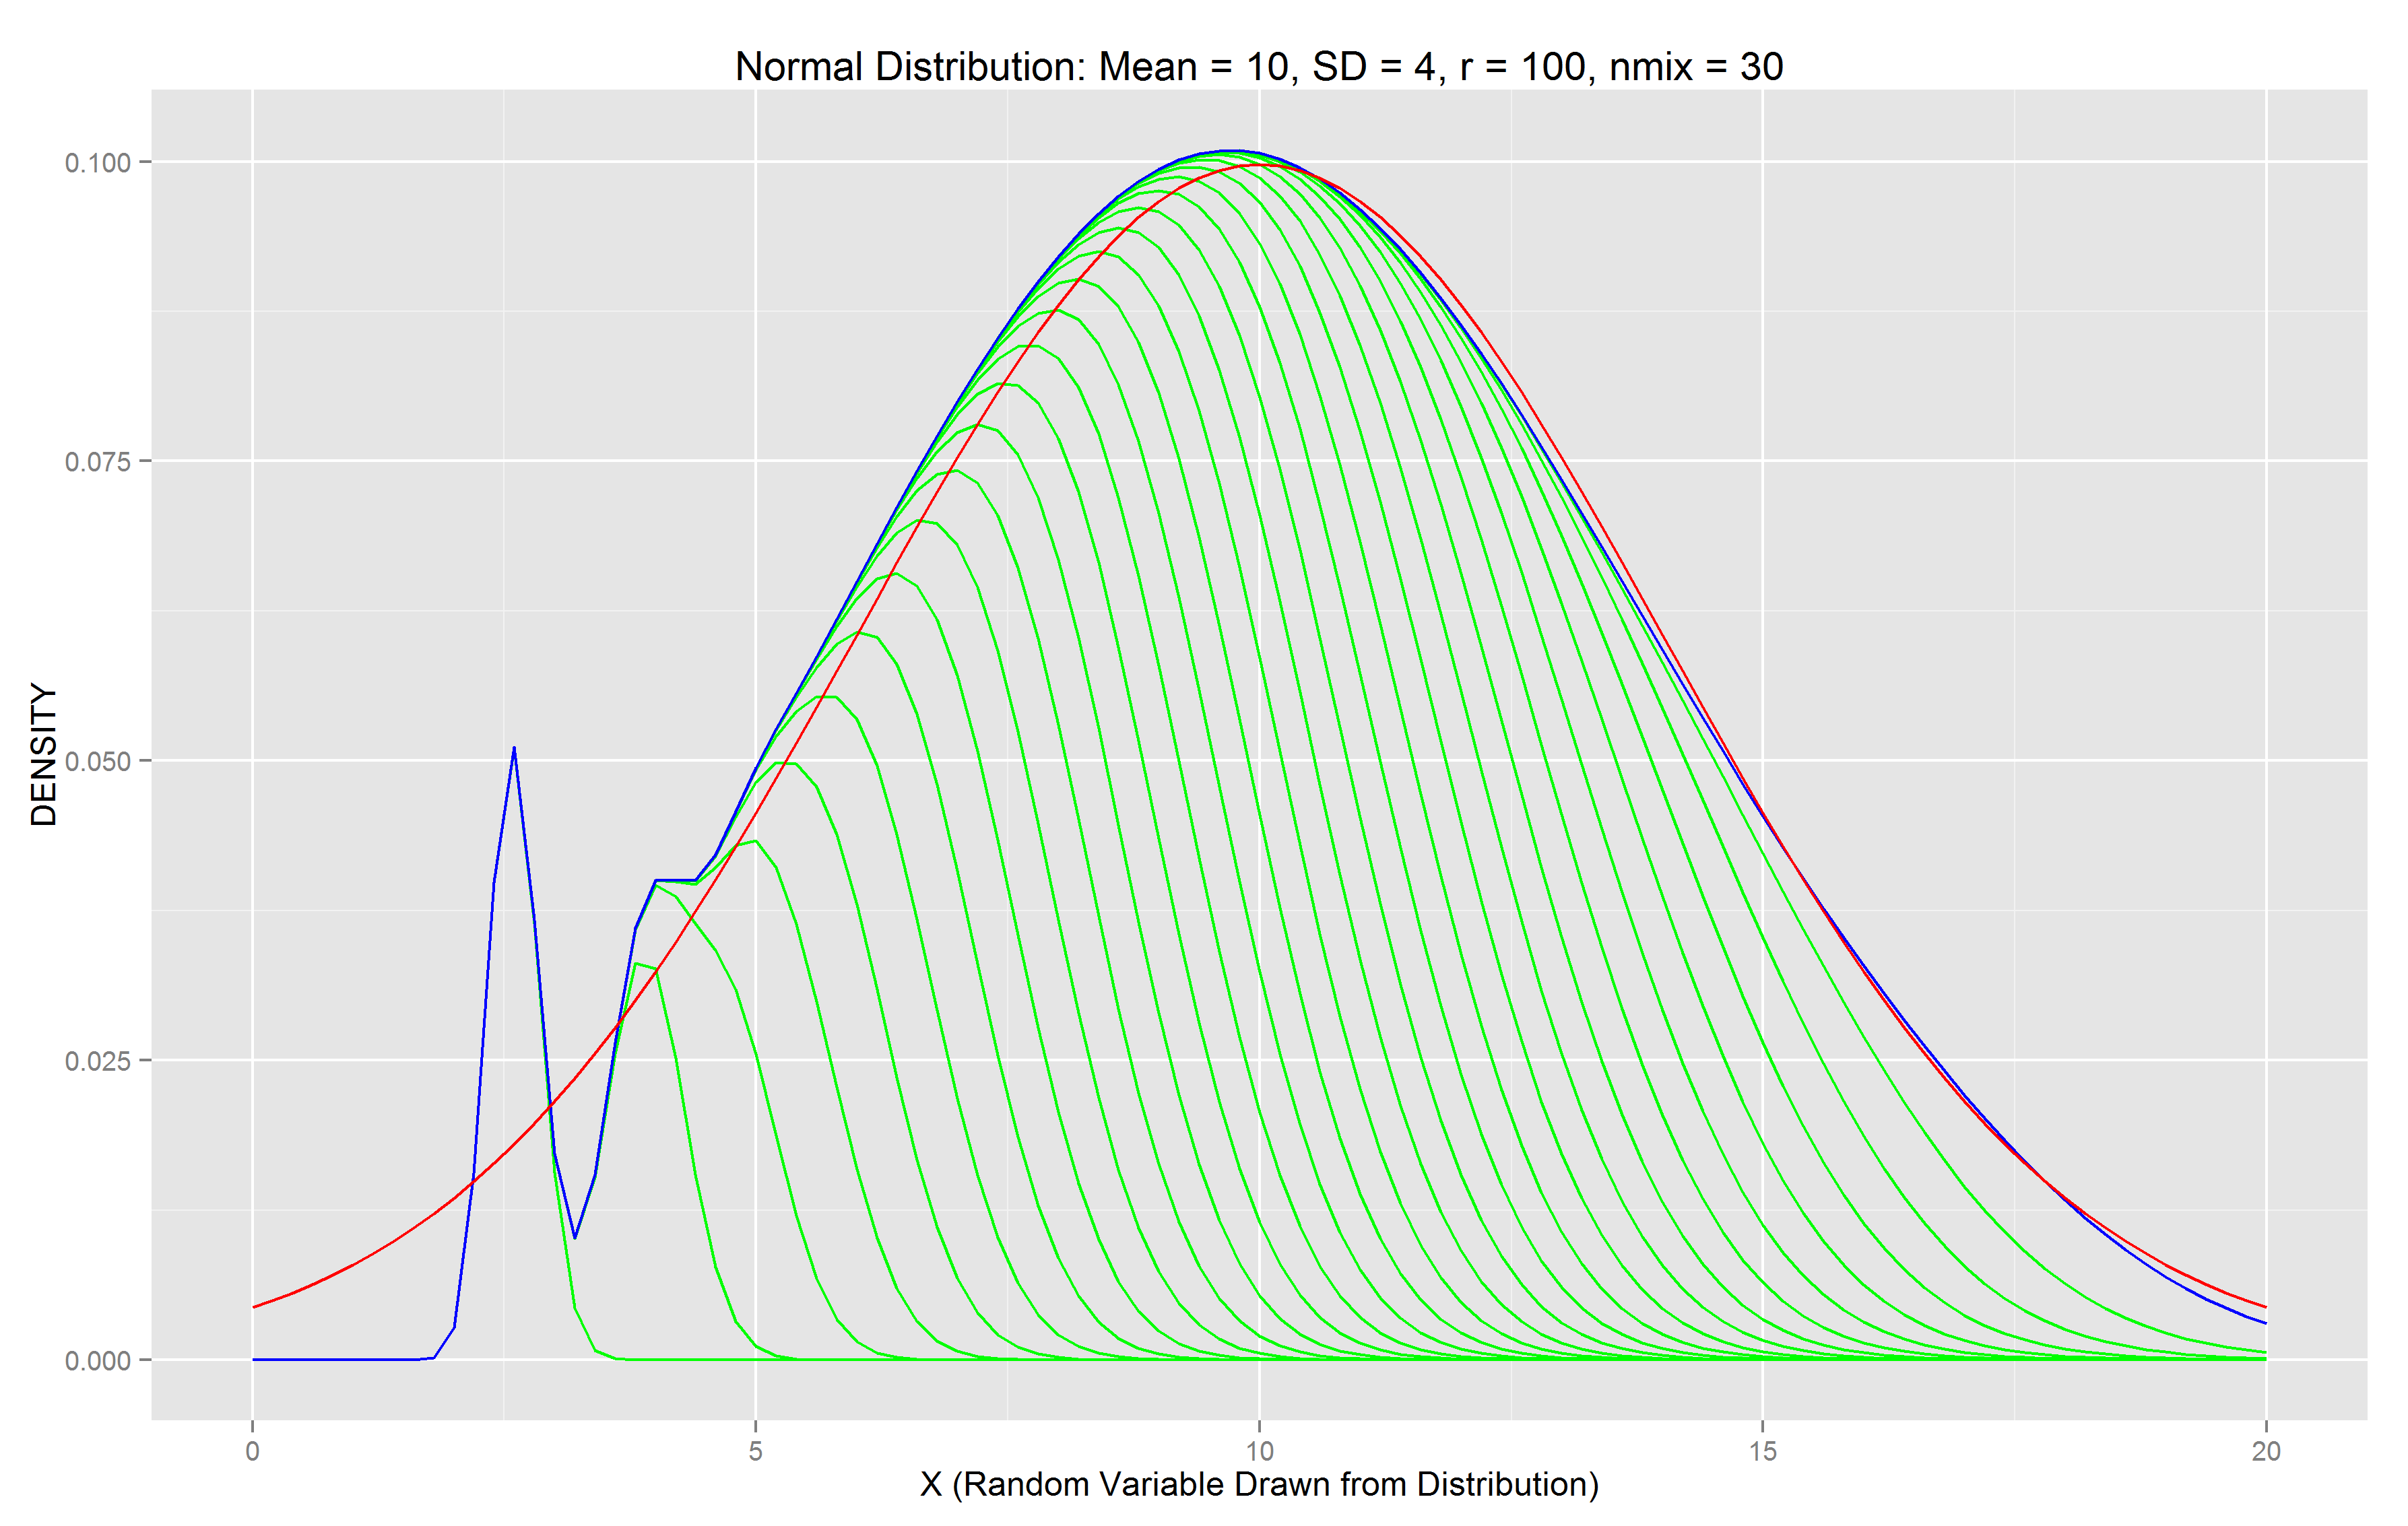
\includegraphics[scale=.27]{normdist_10_4_100_30.png}\\
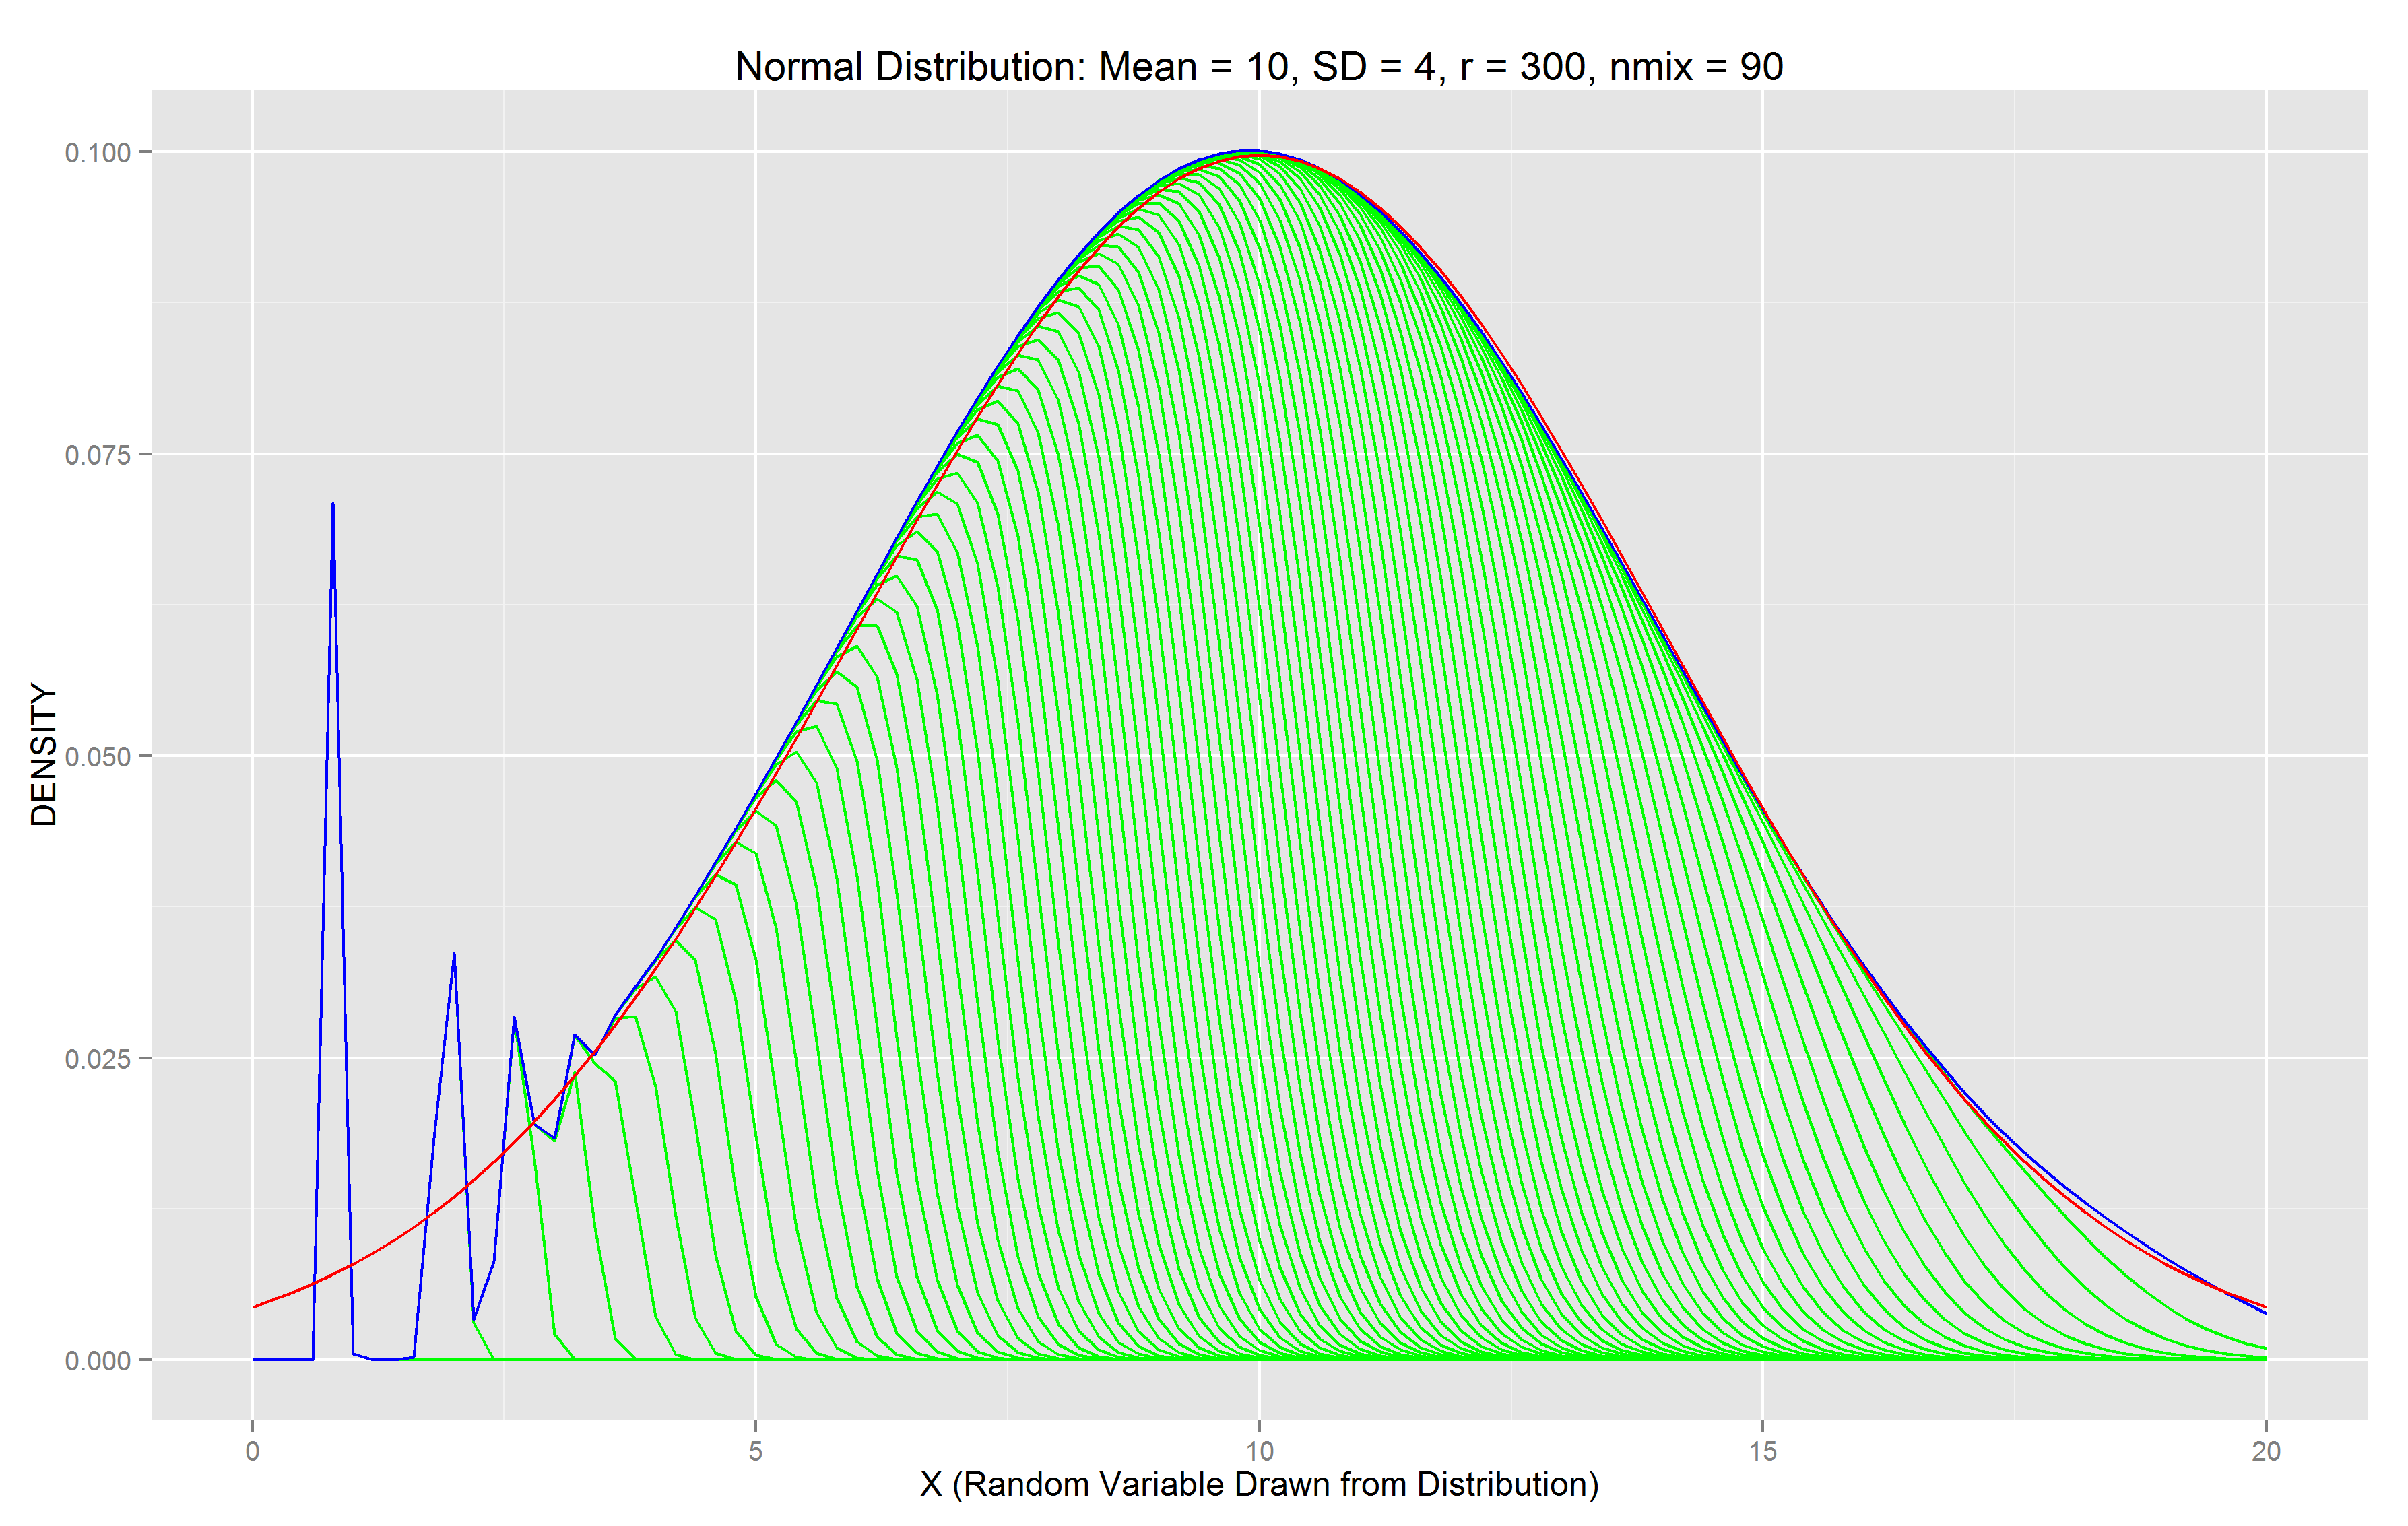
\includegraphics[scale=.54]{normdist_10_4_300_90.png}
\end{figure}

As can be seen, as r 

\newpage

\subsection*{Problem 3.a}
See \texttt{HtoF.R}. 
\lstinputlisting{HtoF.R}


\subsection*{Problem 3.b}
Given a hazard function, $h(t)$, the density function, $f(t)$, can be found as follows:
\begin{equation*}
  \begin{aligned}
      f(t) = h(t) \cdot e^{-\int_0^t \mathrm{h(s)}\,\mathrm{d}s}
  \end{aligned}
\end{equation*}
We looked at the following hazard functions to explore what their density would look like:
\begin{equation*}
  \begin{aligned}
      h(t) &= 5 \\
      h(t) &= 2t \\
      h(t) &= 4 - 2t  \\
      h(t) &= (t-0.5)(t-1)(t-1.5)(t-2) + 0.1\\
  \end{aligned}
\end{equation*}
\begin{figure}[H]
\centering
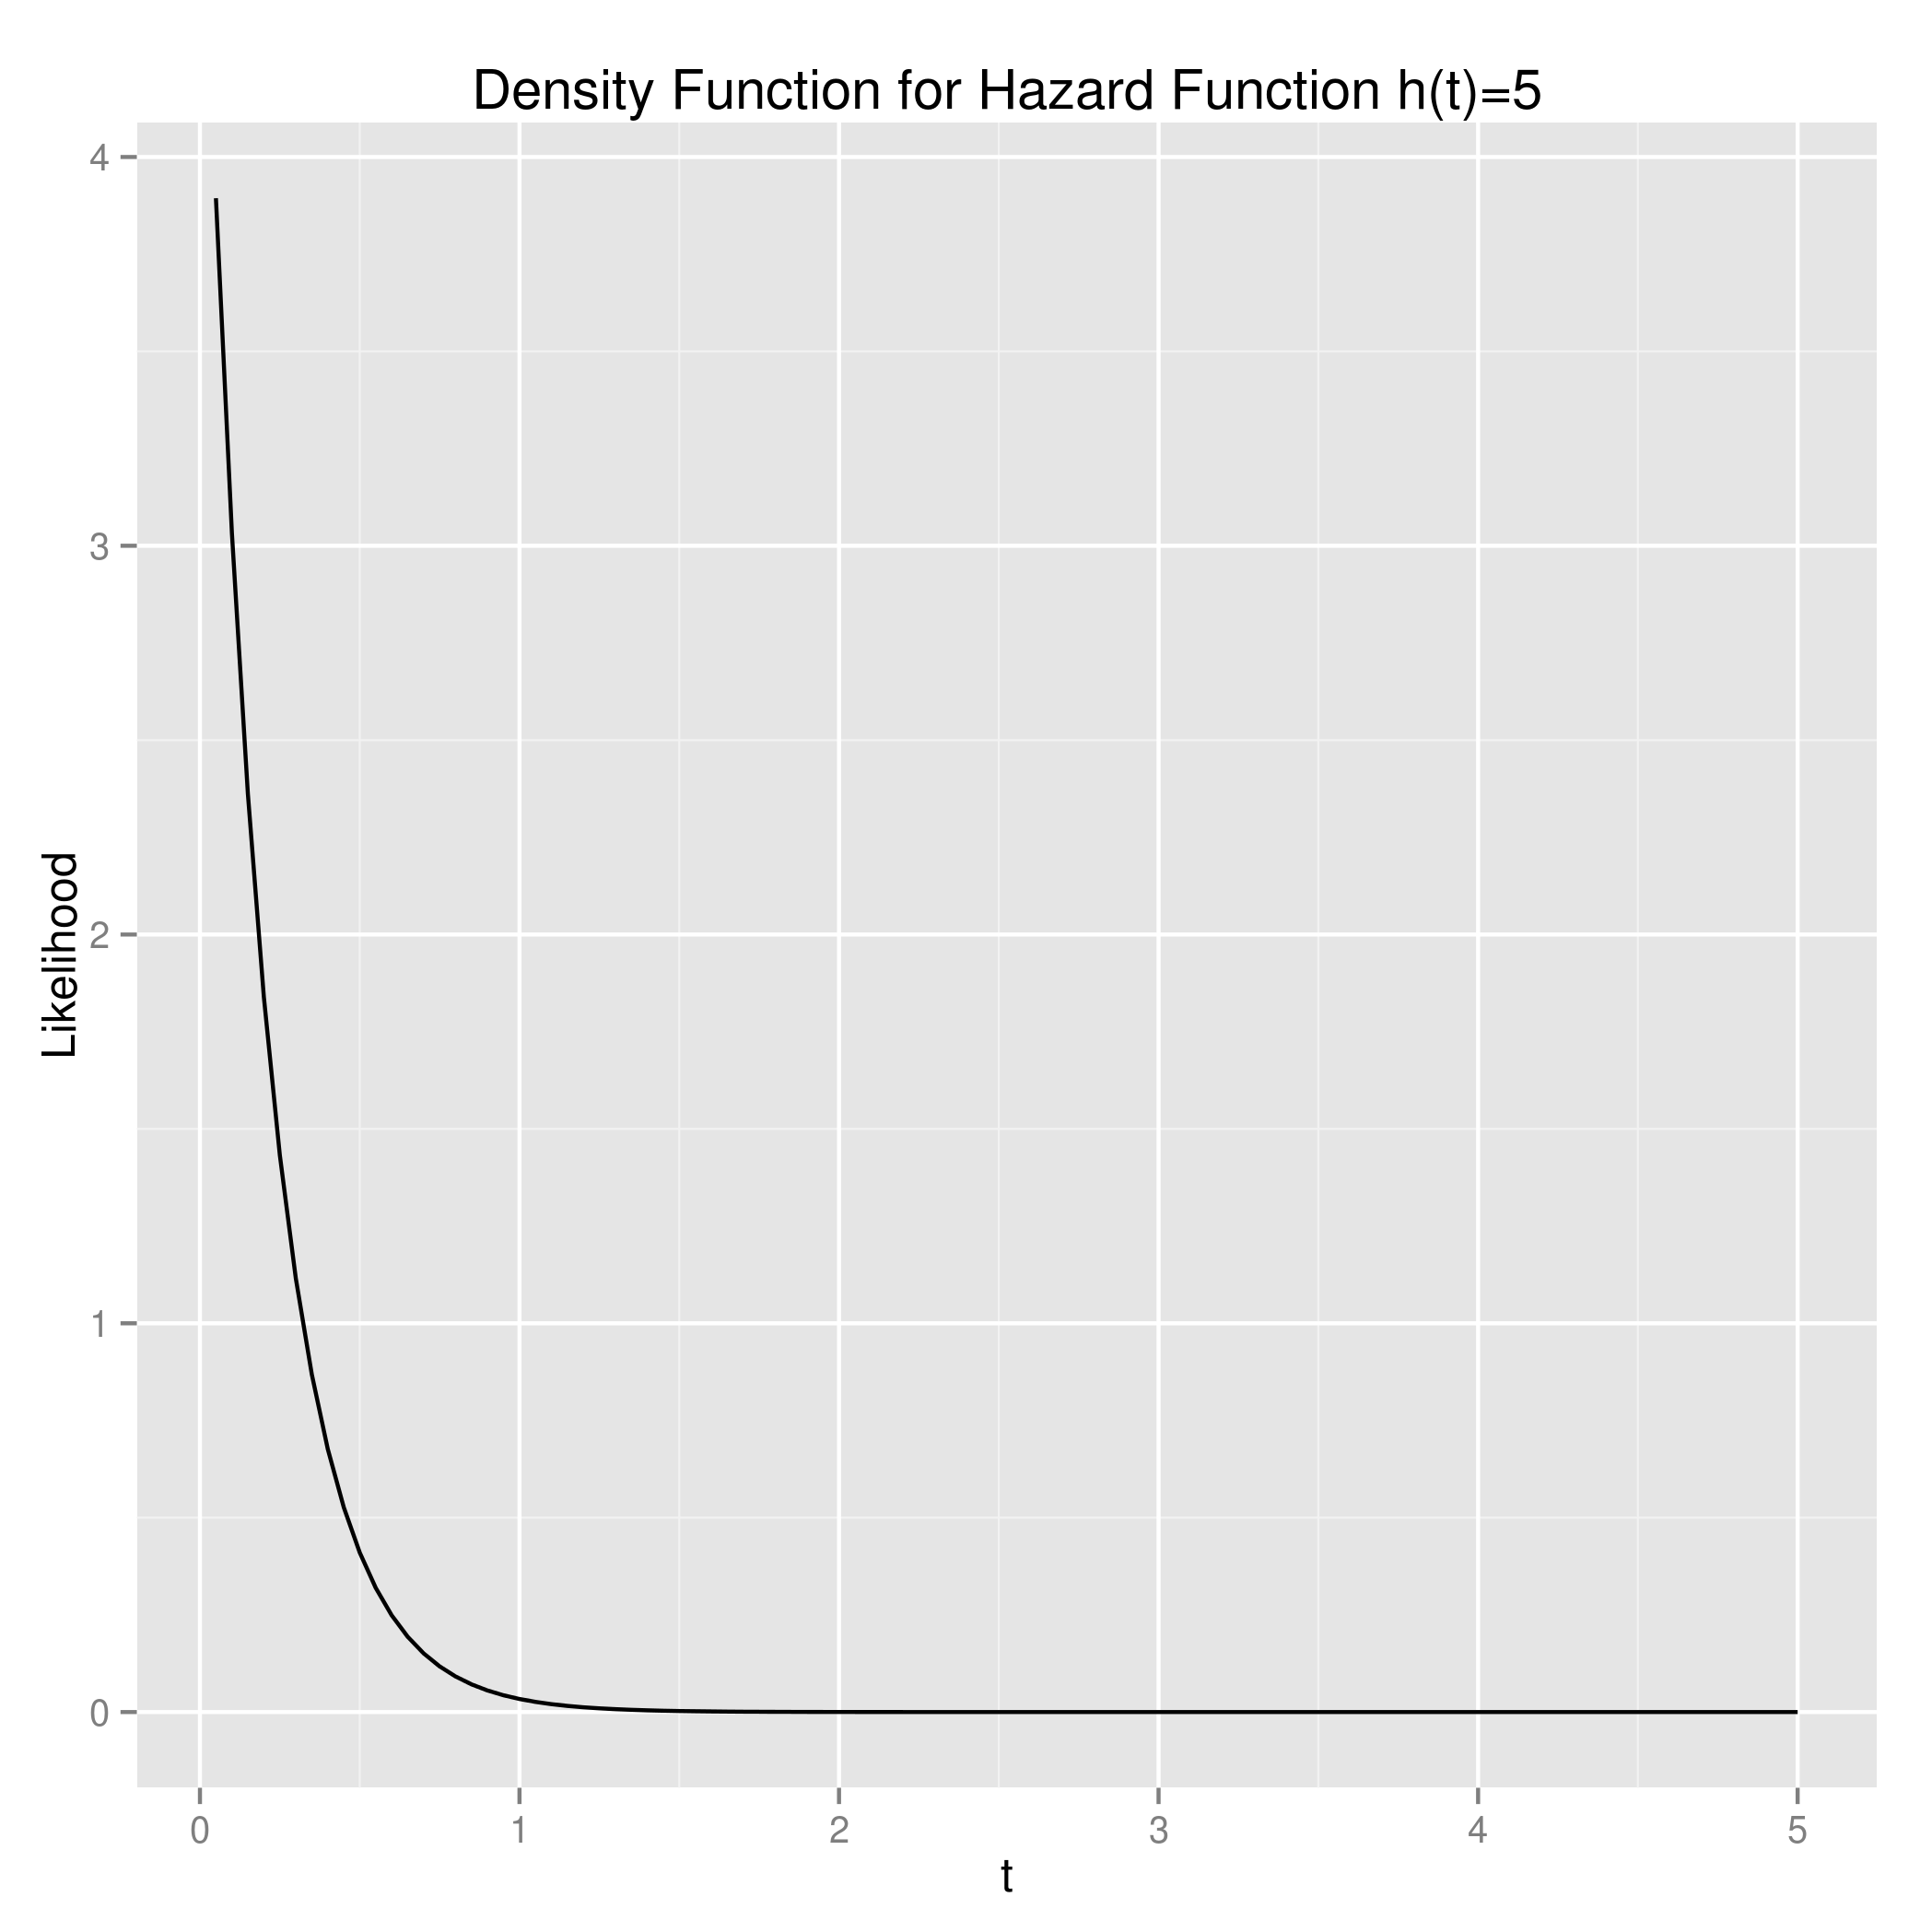
\includegraphics[scale=.33]{3_constant.png}
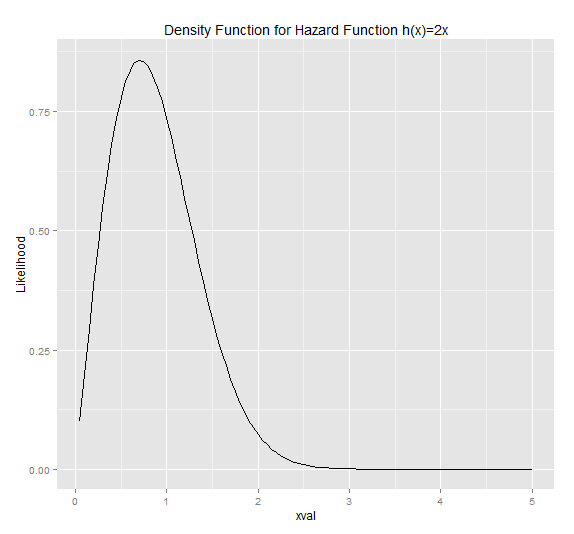
\includegraphics[scale=.33]{3_increasing.png}
\end{figure}
\begin{figure}[H]
\centering
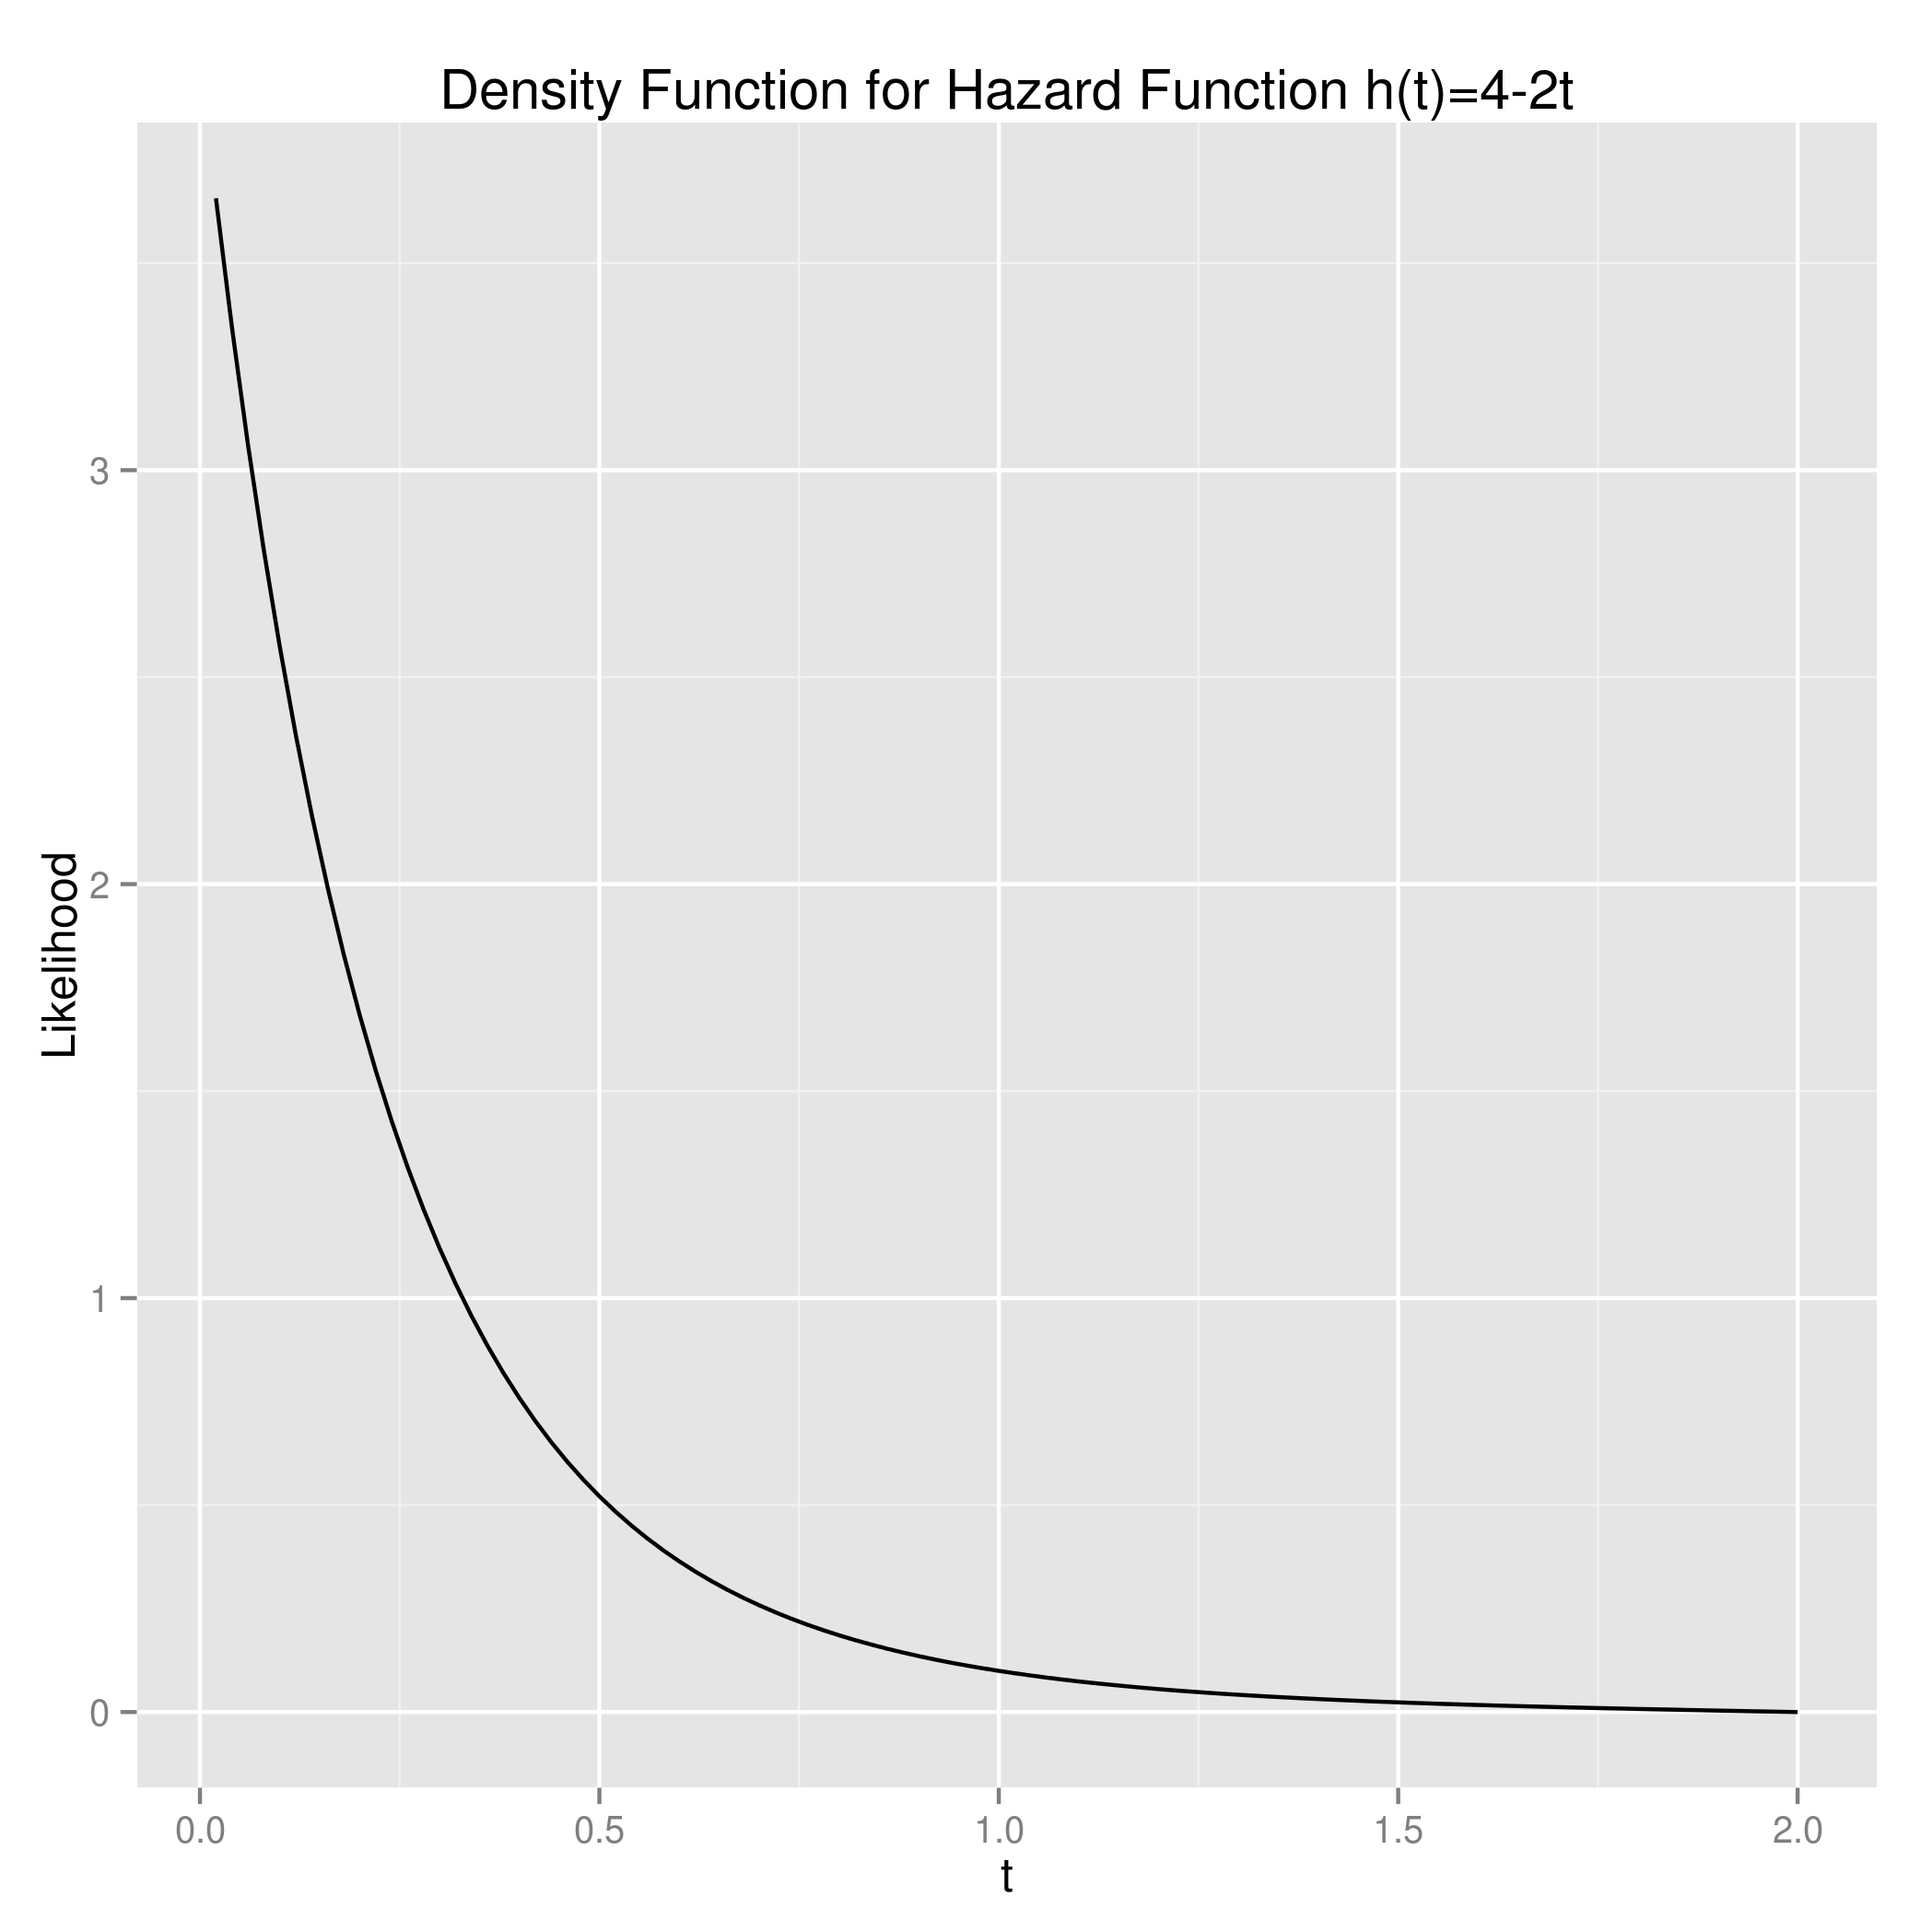
\includegraphics[scale=.33]{3_decreasing.png}
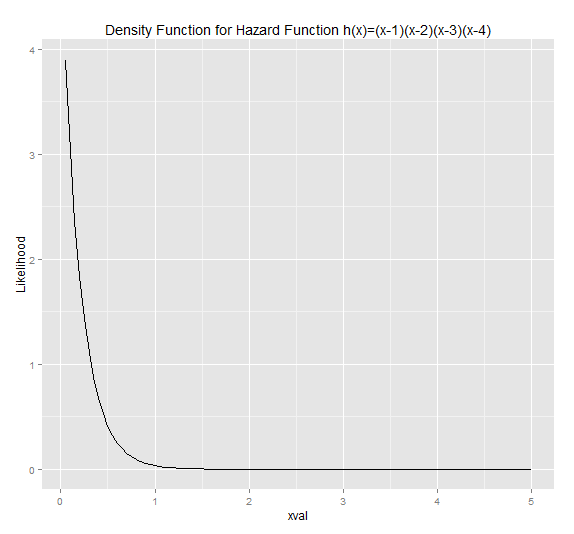
\includegraphics[scale=.33]{3_wshape.png}
\end{figure}
(Plots generated with \texttt{3.R}). 


\subsection*{Problem 4.a-b}

See \texttt{4.R} for generating these plots. 
\begin{figure}[h]
 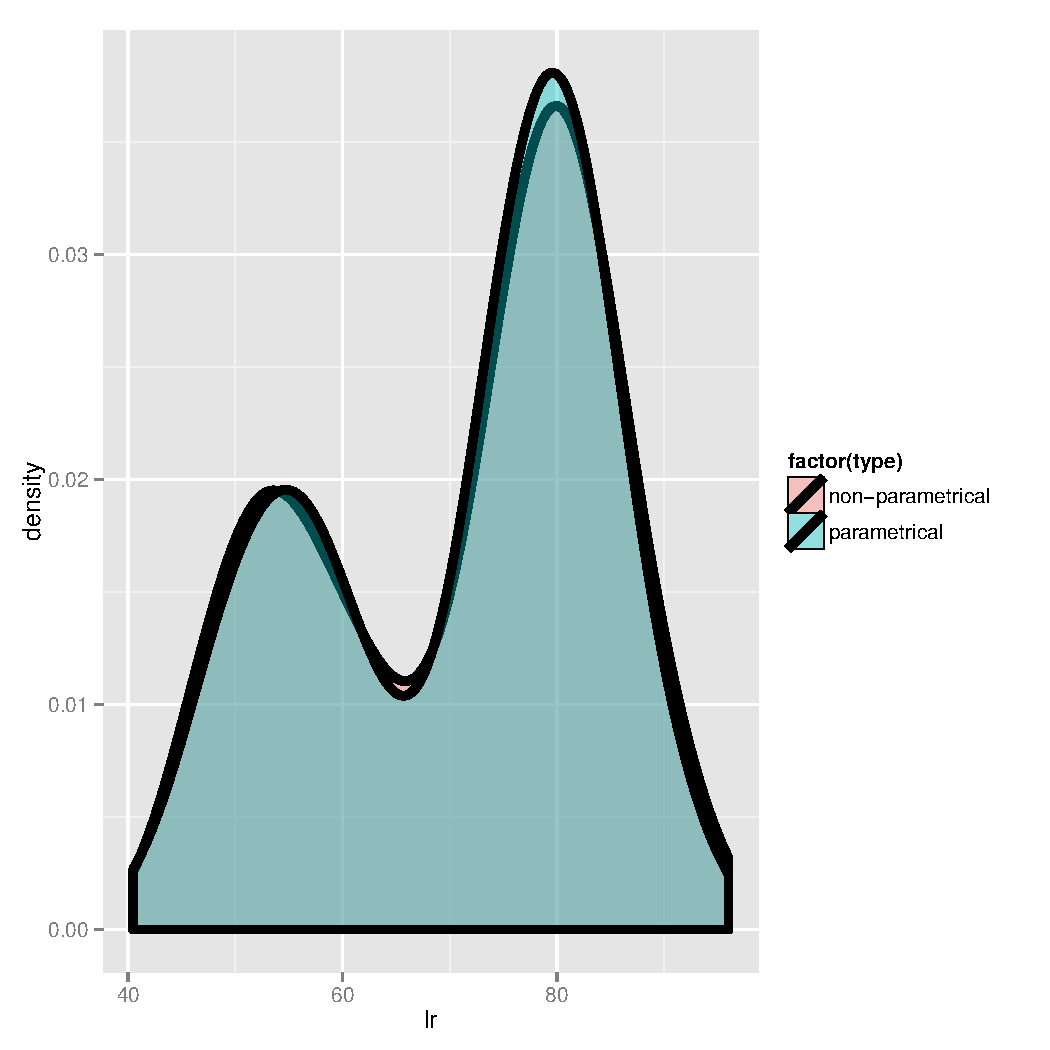
\includegraphics[scale=0.5]{plot4b.pdf}
\end{figure}
\pagebreak



\end{document}
